% https://www.overleaf.com/3817925849trndmfskrvtt
\documentclass[12pt,a4paper]{article}

\usepackage[utf8]{inputenc}
\usepackage[greek,english]{babel}
\usepackage{alphabeta} 

\usepackage{listings}
\usepackage[pdftex]{graphicx}
\usepackage[top=1in, bottom=1in, left=1in, right=1in]{geometry}

\linespread{1.06}
\setlength{\parskip}{8pt plus2pt minus2pt}

\widowpenalty 10000
\clubpenalty 10000

\newcommand{\eat}[1]{}
\newcommand{\HRule}{\rule{\linewidth}{0.5mm}}

\usepackage[official]{eurosym}
\usepackage{enumitem}
\setlist{nolistsep,noitemsep}
\usepackage[hidelinks]{hyperref}
\usepackage{cite}
\usepackage{lipsum}
\usepackage{hyperref}
\hypersetup{
    colorlinks=true,
    linkcolor=blue,
    filecolor=magenta,      
    urlcolor=cyan,
    pdftitle={Overleaf Example},
    pdfpagemode=FullScreen,
    }


\begin{document}

%===========================================================
\begin{titlepage}
\begin{center}

% Top 

\includegraphics[width=0.35\textwidth]{kgp_logo.png}~\\[2cm]


% Title
\HRule \\[0.4cm]
{ \LARGE 
  \textbf{Lab Report for Group Sekhmet}\\[0.4cm]
  \emph{\href{https://sekhmet.vercel.app/}{Hospital Management System}}\\[0.4cm]
}
\HRule \\[1.5cm]



% Author
{ \large
  Srishty Gandhi(20CS30052), Yatindra Indoria (20CS30060) \\
  Chirag Ghosh (20CS10020), Sarita Singh (20CS10053)\\
  Shreya Agrawal (20CS10058) 
}



\vfill

%\textsc{\Large Cyprus University of Technology}\\[0.4cm]
\textsc{\large DBMS LABORATORY\\ \href{https://cse.iitkgp.ac.in}{Department of Computer Science and Engineering} }\\[0.4cm]


% Bottom
{\large \today}
 
\end{center}
\end{titlepage}

% \begin{abstract}
% \lipsum[1-2]
% \addtocontents{toc}{\protect\thispagestyle{empty}}
% \end{abstract}

\newpage



% %===========================================================
% \tableofcontents
% \addtocontents{toc}{\protect\thispagestyle{empty}}
% \newpage
% \setcounter{page}{1}

% %===========================================================
% %===========================================================
% \section*{ \hspace{70 mm}Question-1}
% \section*{ \hspace{-2mm}Design of Ripple Carry Adders }

% \begin{enumerate}
% \item \textbf{Half Adder} \\
% A half adder is a type of adder, an electronic circuit that performs the addition of numbers. The half adder is able to add two single binary digits and provide the output plus a carry value. It has two inputs, called A and B, and two outputs S (sum) and C (carry). \\

% \begin{figure}[htp]
%     \centering
%     \includegraphics[width=10cm]{half_adder_circuit.png}
%     \caption{Half Adder Circuit Diagram}
% \end{figure}

% \textbf{Truth Table:}
% \begin{figure}[htp]
%     % \centering
%   \hspace{9mm} \includegraphics[width=0.5\textwidth]{half_adder_tt.png}
% \end{figure}

% \textbf{Logic} \\
% \(carry = a \& b\) \\
% \(sum = a \oplus b \) \\ \\

% \item \textbf{Full Adder} \\
% Full adder A full adder is a digital circuit that performs addition. Full adders are implemented with logic gates in hardware. A full adder adds three one-bit binary numbers, two operands and a carry bit. The adder outputs two numbers, a sum and a carry bit.\\
% \begin{figure}[htp]
%     \centering
%     \includegraphics[width=10cm]{full_adder_circuit.png}
%     \caption{Full Adder Circuit Diagram}
% \end{figure} \\

% \textbf{Truth Table:}\\ \\
% \begin{figure}[htp]
%     \centering
%     \includegraphics[width=0.8\textwidth]{full_adder_tt.png}
% \end{figure}

% \textbf{Logic} \\\\
% \(carry = a.b + b.c\_in + c\_in.b\) \\
% \(sum = a \oplus b \oplus c\_in \) \\\\

% \item \textbf{Ripple carry adder} \\
% \begin{itemize}
% \item we cascade 8 full adders to make an 8 bit RCA
% \item similarly two 8 bit RCA are cascaded to make a 16bit RCA
% \item this is continued till we get an 64 bit RCA made by cascading two 32bit RCA.
% \end{itemize}

% \begin{figure}[htp]
%     \centering
%     \includegraphics[width=1\textwidth]{8rca.png}
%     \caption{8bit Ripple Carry Adder}
% \end{figure}

% \begin{figure}[htp]
%     \centering
%     \includegraphics[width=0.5\textwidth]{16rca.png}
%     \caption{16bit Ripple Carry Adder}
% \end{figure}

	
%   \begin{figure}[htp]
%     \centering
%     \includegraphics[width=0.5\textwidth]{32rca.png}
%     \caption{32bit Ripple Carry Adder}
% \end{figure} 

% \begin{figure}[htp]
%     \centering
%     \includegraphics[width=0.6\textwidth]{64rca.png}
%     \caption{64bit Ripple Carry Adder}
% \end{figure} 

% \item  A Binary Adder-Subtractor is one which is capable of both addition and subtraction of binary numbers in one circuit itself. The operation being performed depends upon the binary value the control signal holds.

% We can calculate the 2’s complement of the given bits (taking them as 2’s complement integer representations). 2’s complement can be calculated by bit-wise inversion of all input bits followed by an addition of ‘1’. We implement the negation for the test purpose by using ~ operator, and we implement the following ‘add 1’ step using the incoming carry of the full-adder. We then perform the usual adder operation, using the Ripple-Carry-Adder, and it results in subtraction.
% \end{enumerate} 
% \vspace{2cm}

% \begin{figure}[htp]
% \textbf{Delay Paths:} \\
%     % \centering
%     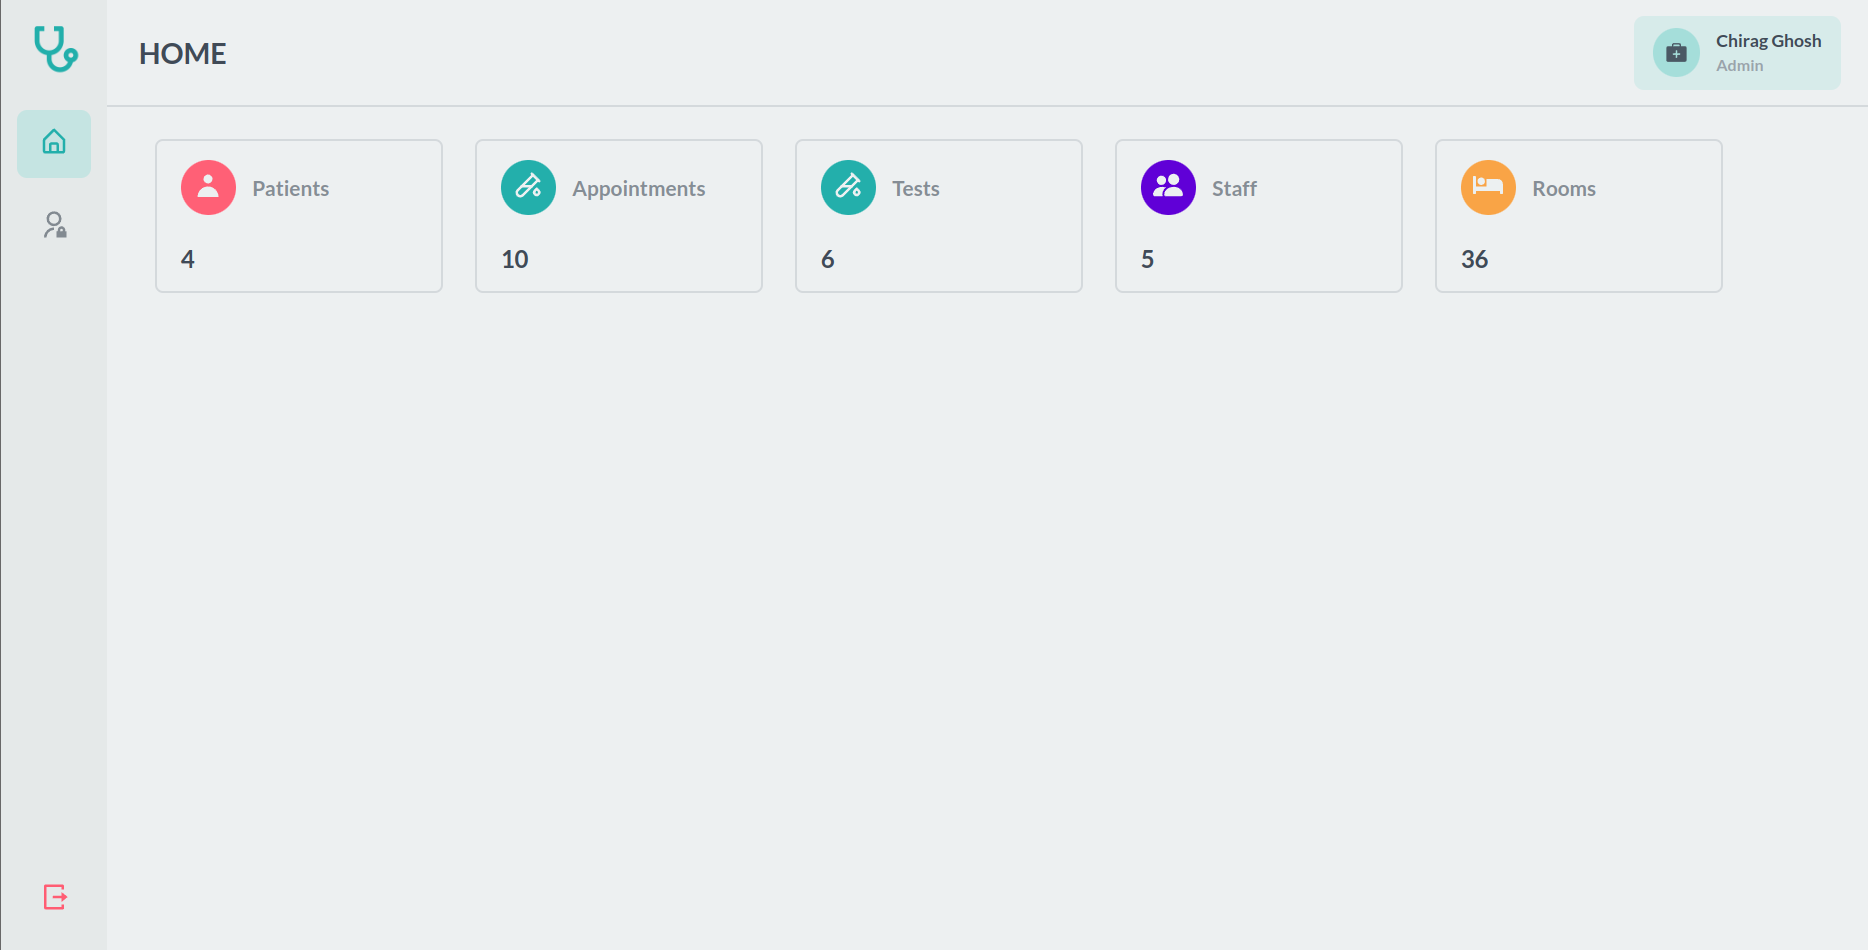
\includegraphics[width=1\textwidth]{image.png}
% \end{figure} 

% \vspace{1.5cm}

% \textbf{File Names:} \\
% \begin{itemize}
% \item \(half\_addr.v ; half\_addr_test.v\)
% \item \(full\_addr.v ; full\_addr\_test.v\)
% \item \(rca\_8\_bit.v ; rca\_8_bit\_test.v\)
% \item \(rca\_16\_bit.v ; rca\_16\_bit\_test.v\)
% \item \(rca\_32\_bit.v , rca_32_bit_test.v\)
% \item  \(rca\_64\_bit.v ; rca\_64\_bit\_test.v ; rca\_64\_bit\_subtract\_test.v\)
% \end{itemize}



% \begin{figure}[htp]
% \textbf{ISE screenshots:} \\ \\
 
%     \includegraphics[width=1\textwidth]{8_sim.png}
%     \caption{8-bit-ISE\_screenshot}
% \end{figure}
% \begin{figure}[htp]
%     \centering
%     \includegraphics[width=1\textwidth]{16_sim.png}
%     \caption{16-bit-ISE\_screenshot}
% \end{figure}

% \begin{figure}[htp]
%     \centering
%     \includegraphics[width=1\textwidth]{32_sim.png}
%     \caption{32-bit-ISE\_screenshot}
% \end{figure}

% \begin{figure}[htp]
%     \centering
%     \includegraphics[width=1\textwidth]{64_sim.png}
%     \caption{64-bit-ISE\_screenshot}
    

% \end{figure}


\section*{ \centerline{\href{https://sekhmet.vercel.app/}{Hospital Management Lab Mini Project }}}
\section*{ \hspace{-2mm}Introduction}
This report outlines the implementation of Flask, Flask Bcrypt, and JWT-based authentication for data security in hospital management system. The system registers patient, schedules appointments with doctors, maintains patient information about diagnostic tests and treatments administered, maintains information about doctors/healthcare professionals, and stores admit/discharge information about the patient. The intended users of the system are front desk operators, data entry operators, doctors and database administrators. Here is the {\href{https://sekhmet.vercel.app/}{link} for our working project.

\section*{ \hspace{-2mm}Backend}


\begin{enumerate}
\item \textbf{Backend written in Flask} 

The backend of the hospital management system has been implemented using Flask, a popular Python-based web framework. Flask provides a lightweight and flexible web application framework, making it an ideal choice for this project.

\\
\\Flask has been used to create the endpoints for registering patients, scheduling appointments with doctors, maintaining patient information about diagnostic tests and treatments administered, maintaining information about doctors/healthcare professionals, and storing admit/discharge information about the patients.
\\

\begin{lstlisting}
@app.route('/user', methods=['POST', 'GET'])
def user():

@app.route('/user/login', methods=['POST', 'GET'])
def user_login():

@app.route('/patient', methods=['POST', 'GET'])
def patient():

@app.route('/patient/<int:ssn>')
def patient_ssn(ssn):

@app.route('/patient/<int:ssn>/appointment', methods=['POST', 'GET'])
def patient_ssn_appointment(ssn):

@app.route('/patient/<int:ssn>/test', methods=['POST', 'GET'])
def patient_ssn_test(ssn):

@app.route('/physician', methods=['POST', 'GET'])
def physician():

@app.route('/physician/<int:id>')
def physician_id(id):

@app.route('/physician/engagements')
def physician_engagements()

@app.route('/procedure')
def procedure():

@app.route('/procedure/<int:id>', methods=['POST'])
def procedure_id(id)

@app.route('/medication')
def medication():

@app.route('/appointment/<int:id>', methods=['PATCH', 'GET'])
def appointment_id(id):

@app.route('/notify')
def notify():

@app.route('/stats')
def stats():


\end{lstlisting}

\\

\item \textbf{Flask-Bcrypt used for password hashing} 

Flask-Bcrypt has been used for password hashing, which is an essential step in data security. Flask-Bcrypt is a library that provides hashing utilities for Flask, by instantiating a 'Bcrypt' object, making it easy to generate and validate secure password hashes.
\begin{figure}[htp]
    \centering
    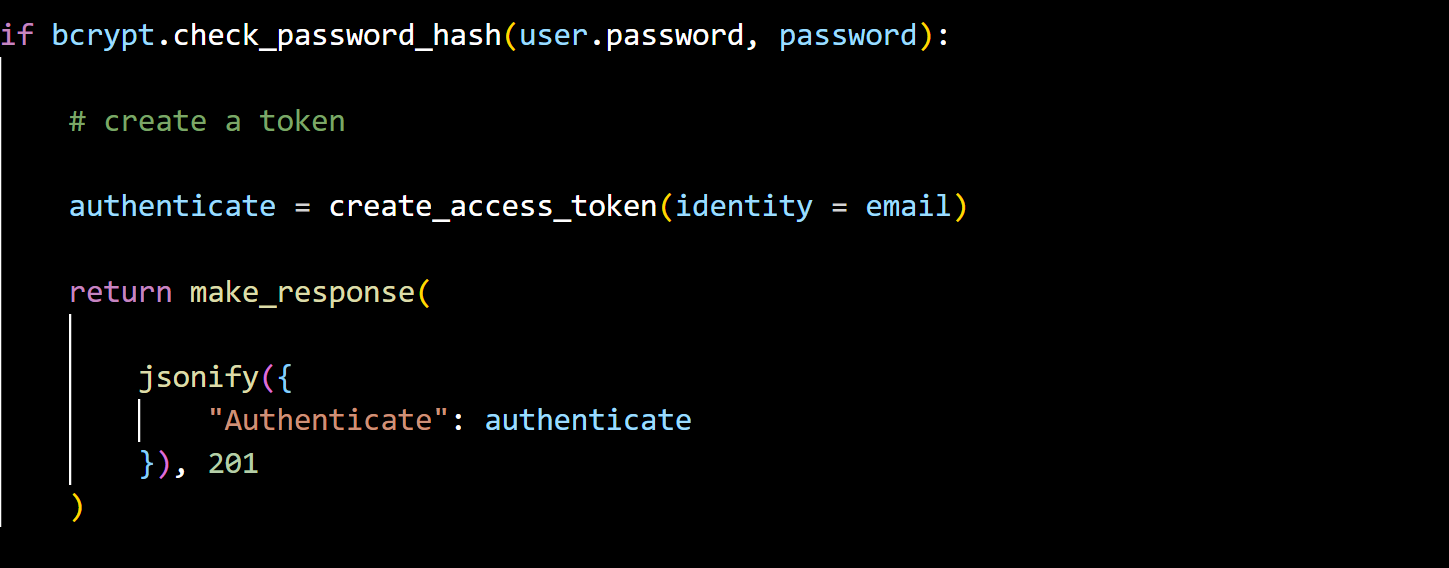
\includegraphics[width=0.6\textwidth]{routes.py - Sekhmet [WSL_ Ubuntu] - Visual Studio Code 12-03-2023 21_34_11.png}
    \caption{Password Hashing using Bcrypt}
\end{figure}

\\ Passwords for all users including front desk operators, data entry operators, doctors, and database administrators are hashed before being stored in the database.
\\
\item \textbf{JWT-based authentication implemented for data security} 

To further improve data security, JWT-based authentication has been implemented. JWT-based authentication allows users to authenticate themselves without sending their passwords over the network, reducing the risk of password theft. JWTs are cryptographically signed tokens that can be used to authenticate users. Only authenticated users can perform certain operations such as scheduling appointments, entering patient data about tests and treatments and querying patient information
\\

\begin{figure}[htp]
    \centering
    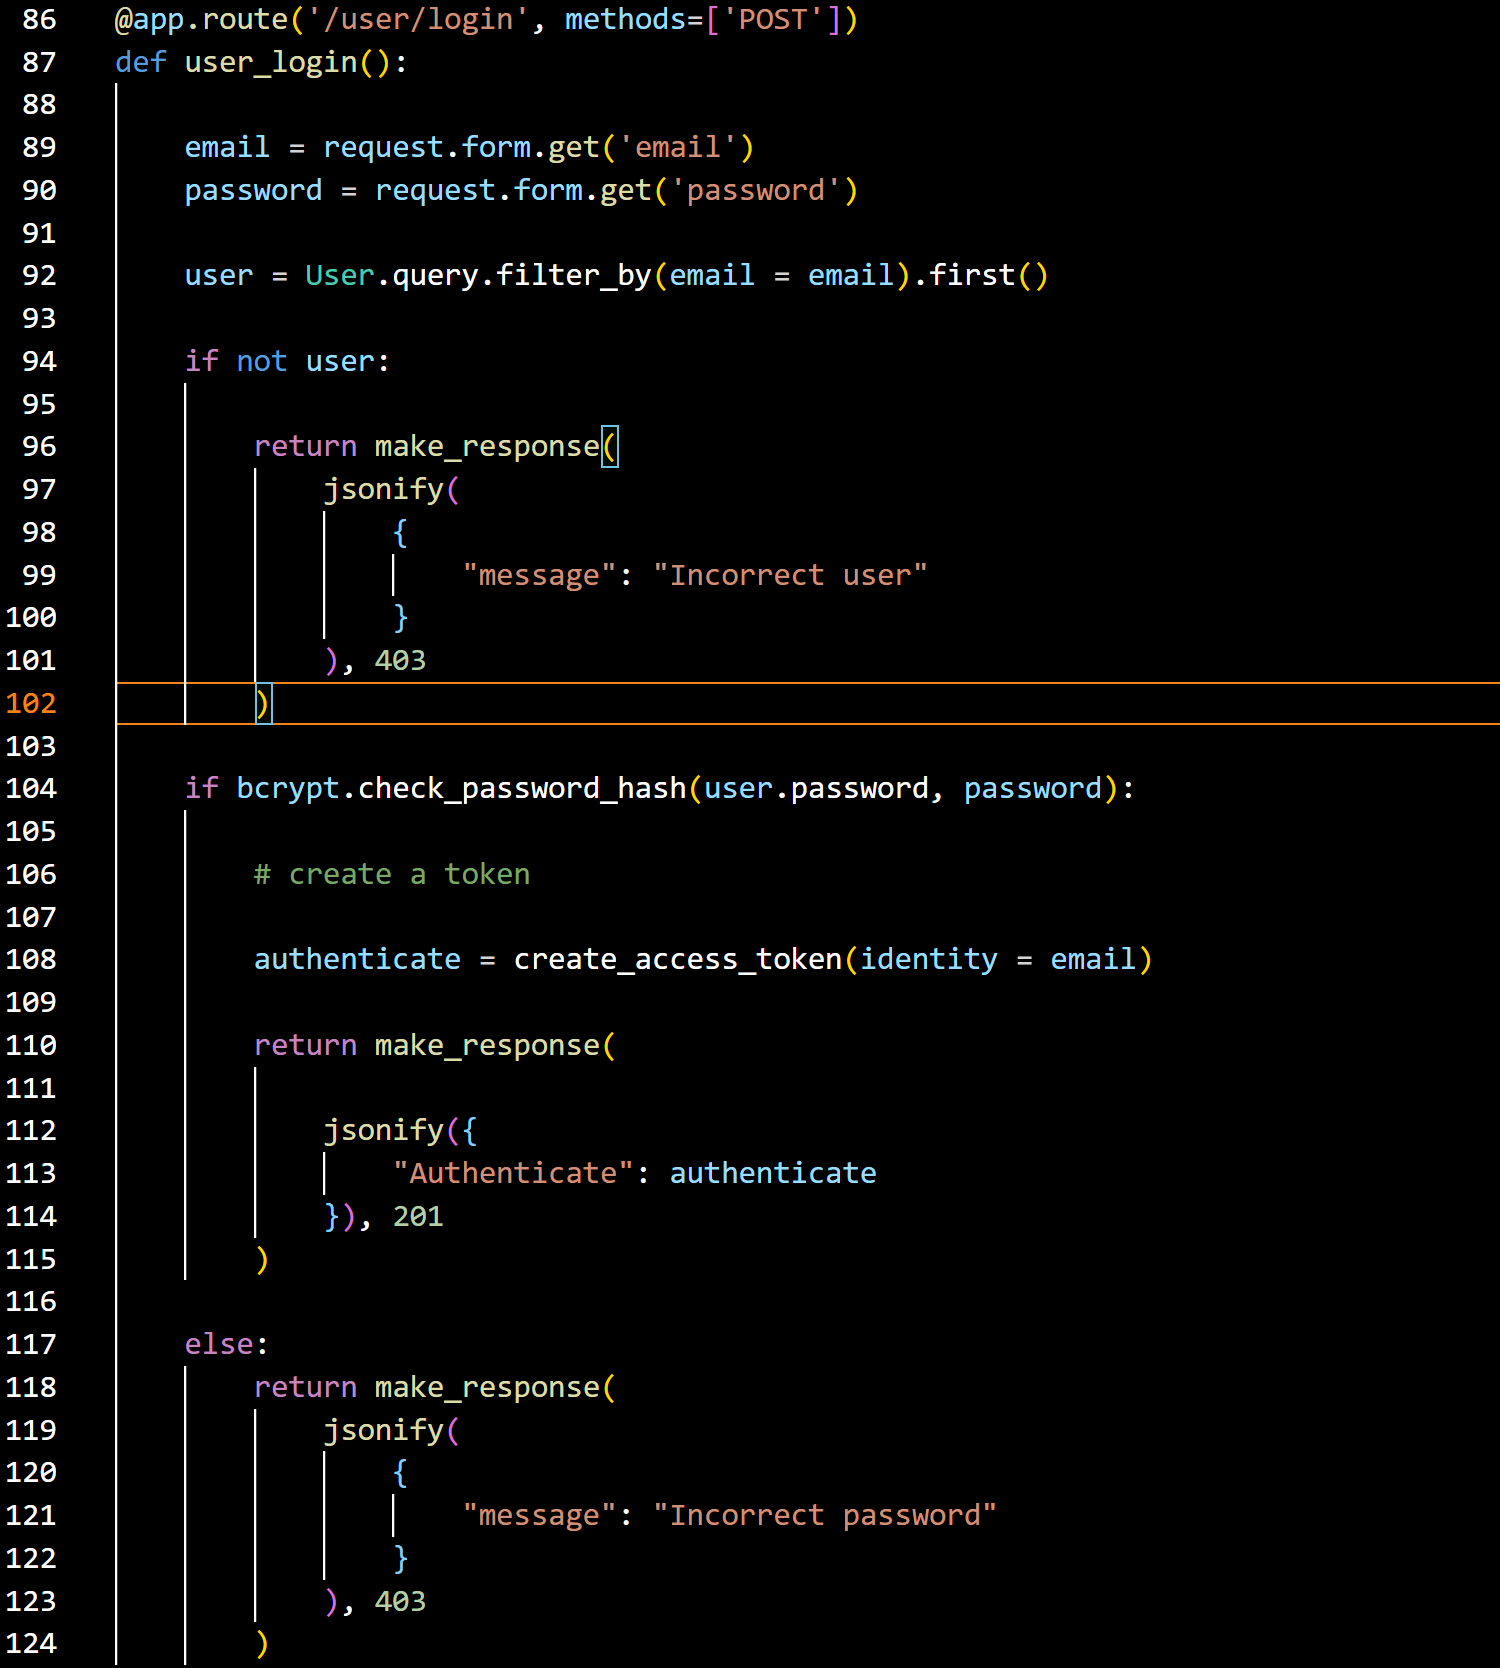
\includegraphics[width=0.6\textwidth]{login_code_jwt.png}
    \caption{Role-based login using JWT}
\end{figure}
\item \textbf{Role-based authentication } 

Role-based authentication has been added to the frontend, allowing users to authenticate themselves based on their roles. This adds an additional layer of security to the application, ensuring that only authorized users can access sensitive data. Front desk operators can only register, admit, and discharge patients, while data entry operators can only enter patient data about tests and treatments. Doctors can query patient information, but cannot modify or delete it. Database administrators have the authority to add or delete users

\begin{figure}[htp]
    \centering
    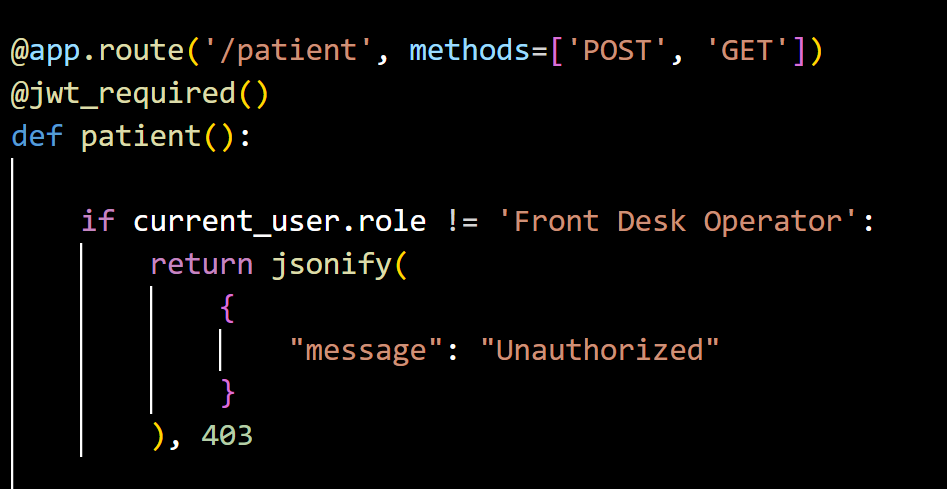
\includegraphics[width=0.6\textwidth]{role_based.png}
    \caption{Role-based authentication for a route}
\end{figure}

\newpage

\item \textbf{Changes made to database} 

The undergoes table in the database has been modified to include two new attributes - results and artifact. Results attribute is used to store the result of the procedure, while the artifact attribute is used to store images such as X-rays related to the procedure. This modification was made to provide a comprehensive record of the patient's diagnosis and treatment.
\\
\item \textbf{Triggers implemented} 

A trigger has been added to automate the patient registration process. When a patient is added to the patient table, the trigger automatically looks up for an empty room from the room table and updates it as occupied. Along with that, it updates the stay table as well. This modification was made to ensure that the patient's stay in the hospital is recorded accurately, reducing the risk of human error and ensuring that the patient is assigned a room quickly.
\\

\end{enumerate}
\section*{ \hspace{-2mm}Frontend}

\begin{enumerate}
\item \textbf{Role based UI}

We implemented different UI on the basis of roles like Doctor, Admin, Front Desk Operator and Data Entry Operator. We ensured that a person cannot access unauthorized data by simply changing the URLs. As the backend will return a '403: Unauthorized Error` in case of a user-role mismatch. The same is ensured by keeping the Role state of the 'current-user'.
\\
Here are the screenshots attached displaying the UI for different roles.
\\

\begin{figure}[htp]
    \centering
    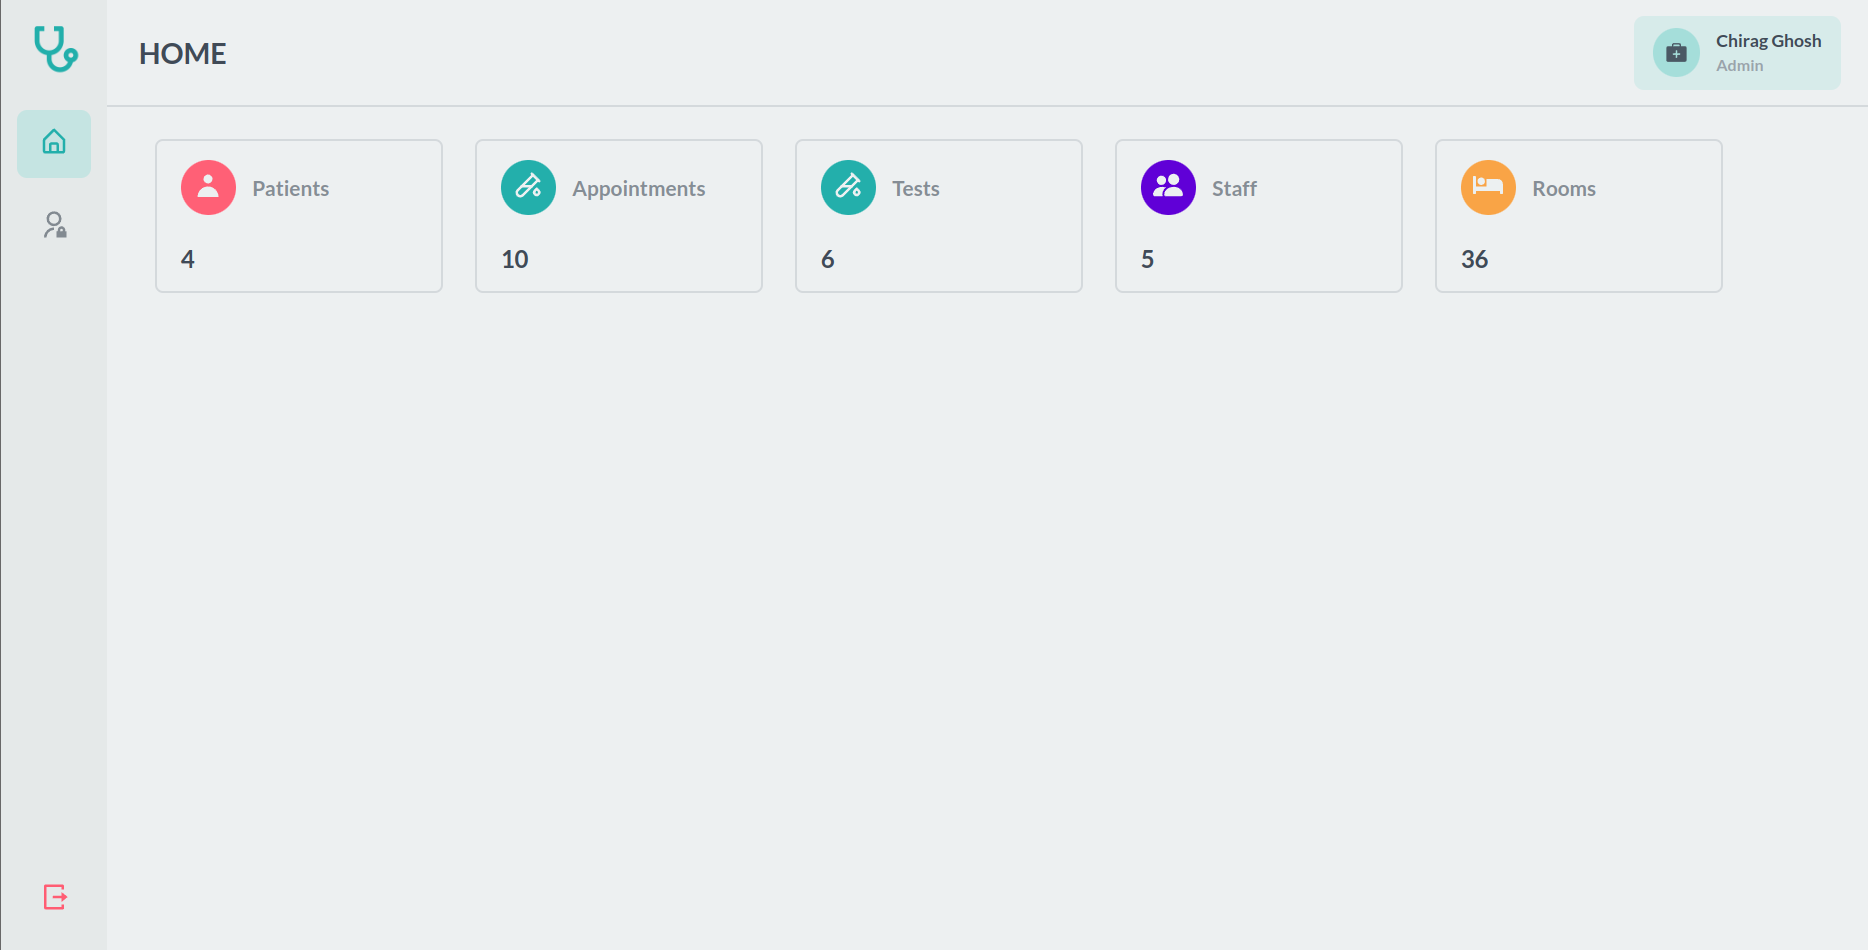
\includegraphics[width=1\textwidth]{image.png}
    \caption{Common Landing page}
\end{figure}
\begin{figure}[htp]
    \centering
    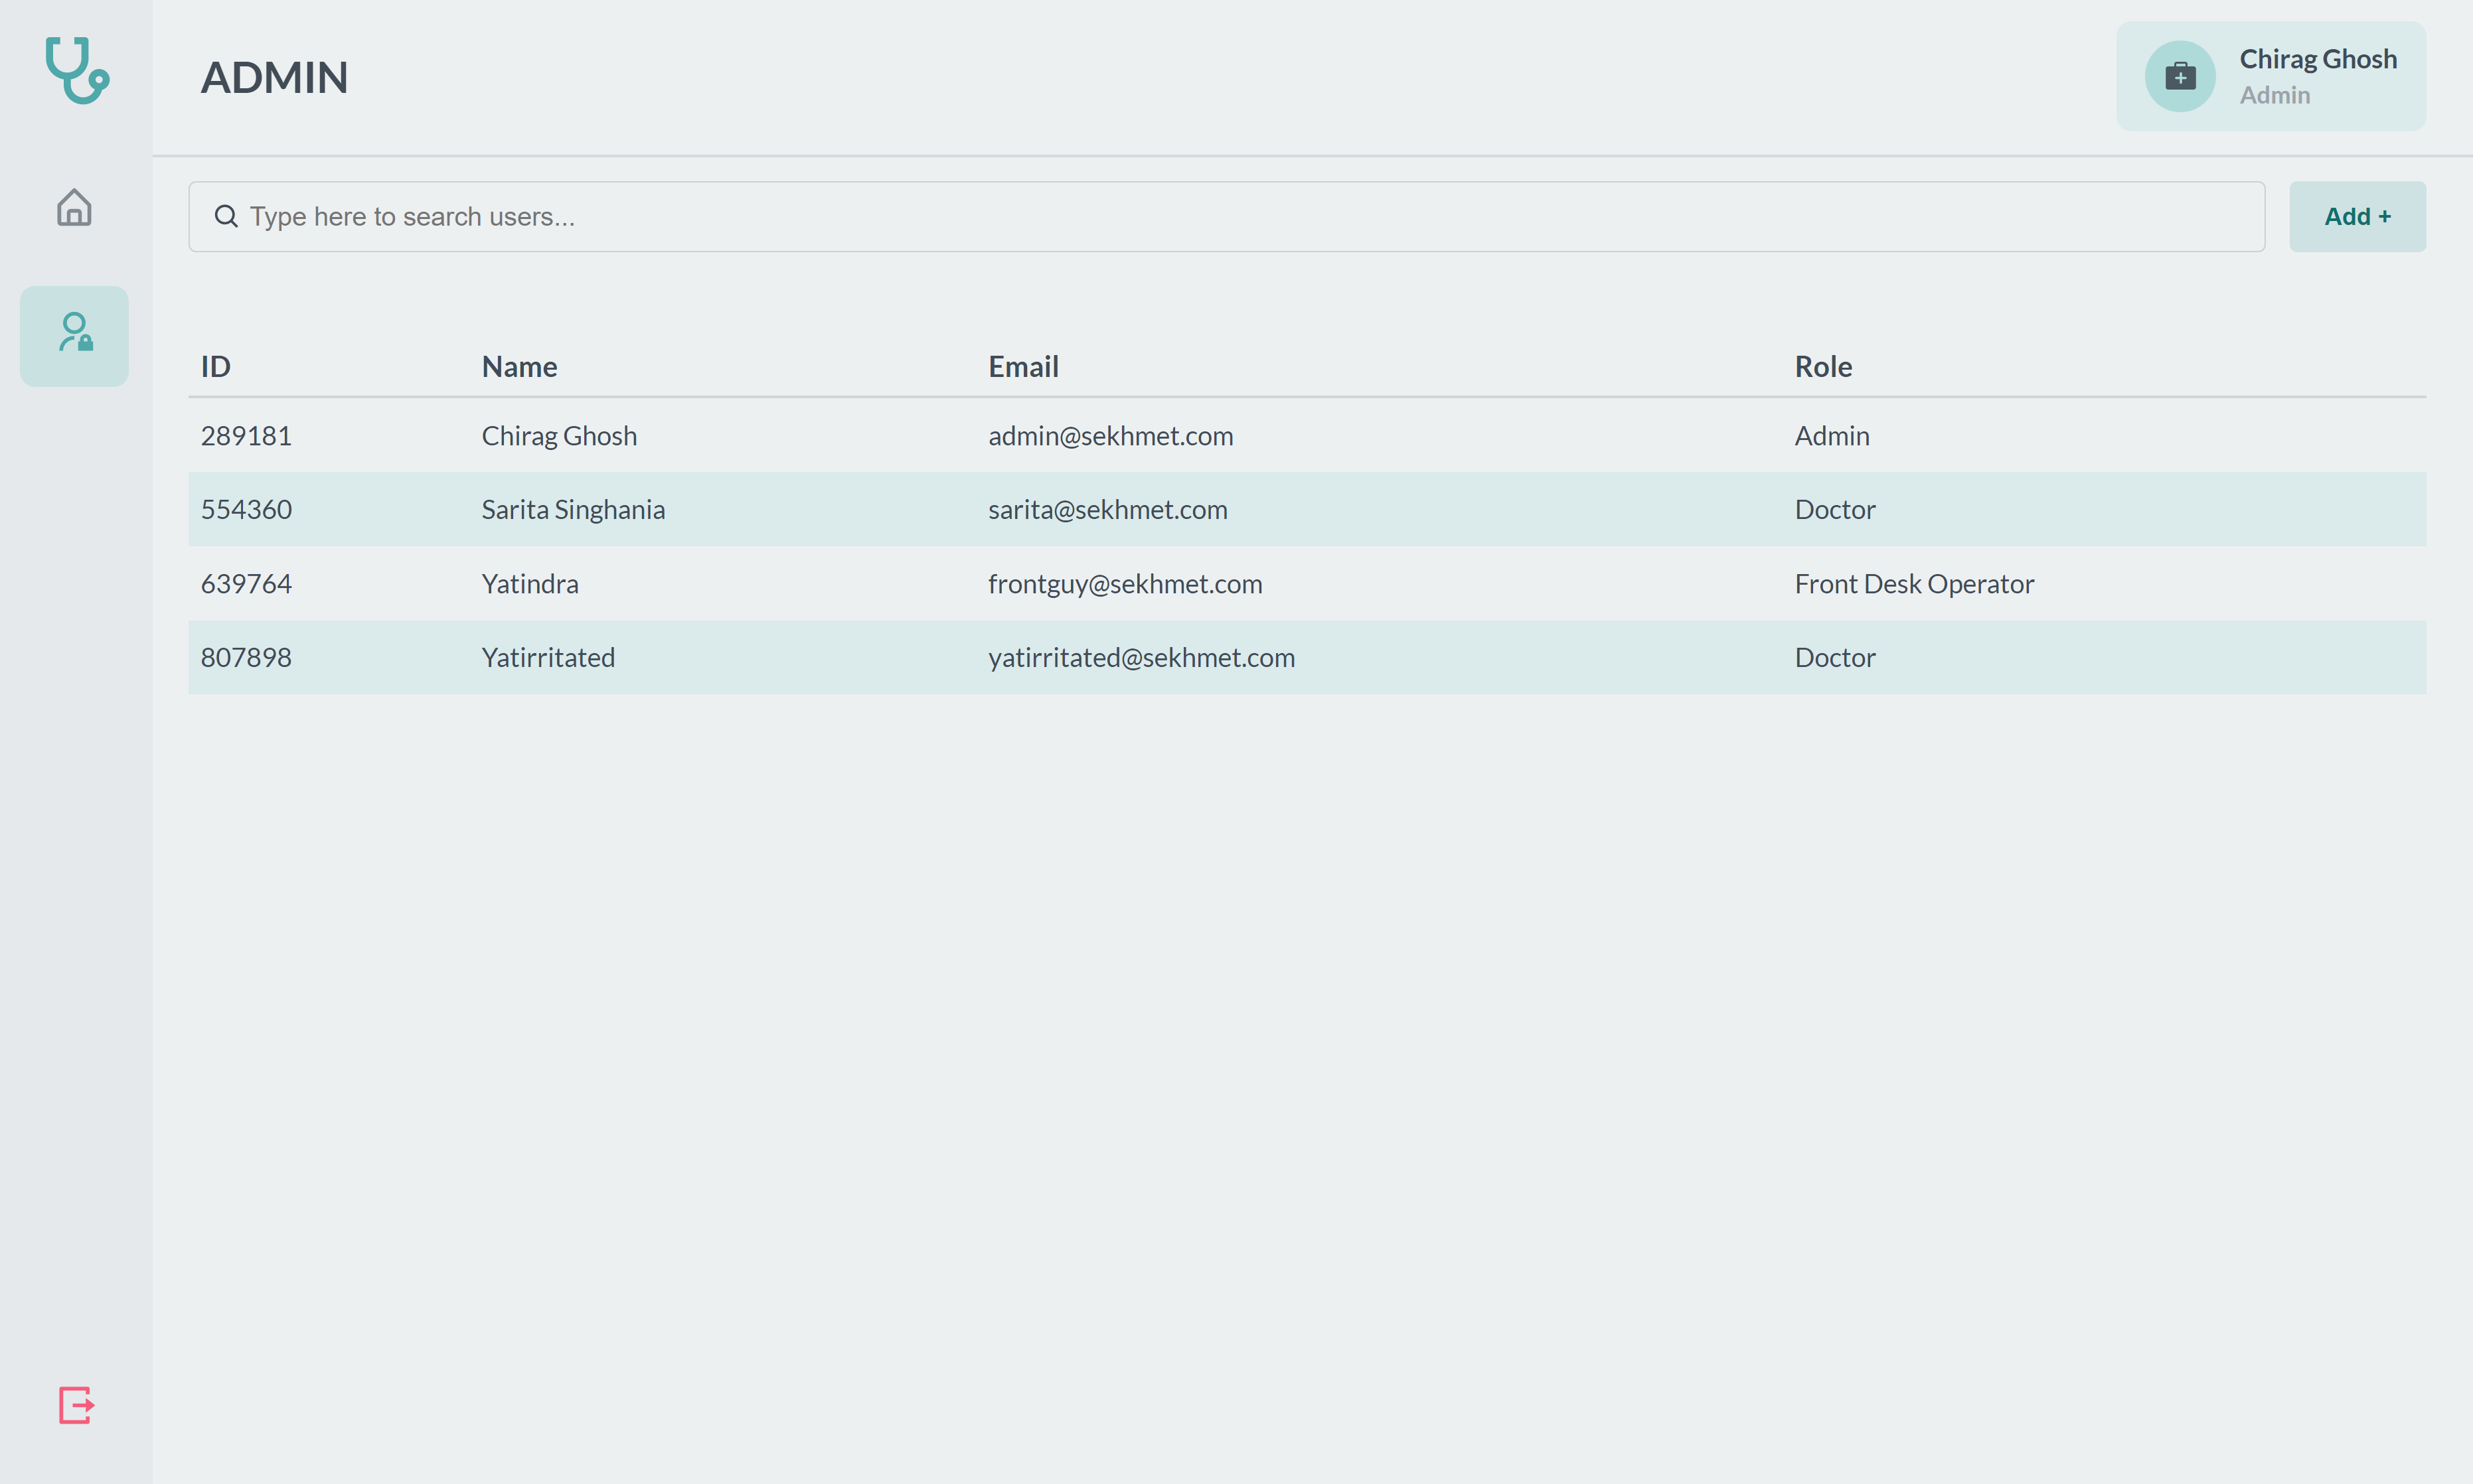
\includegraphics[width=1\textwidth]{admin_console.png}
    \caption{Admin Page}
\end{figure}
\begin{figure}[htp]
    \centering
    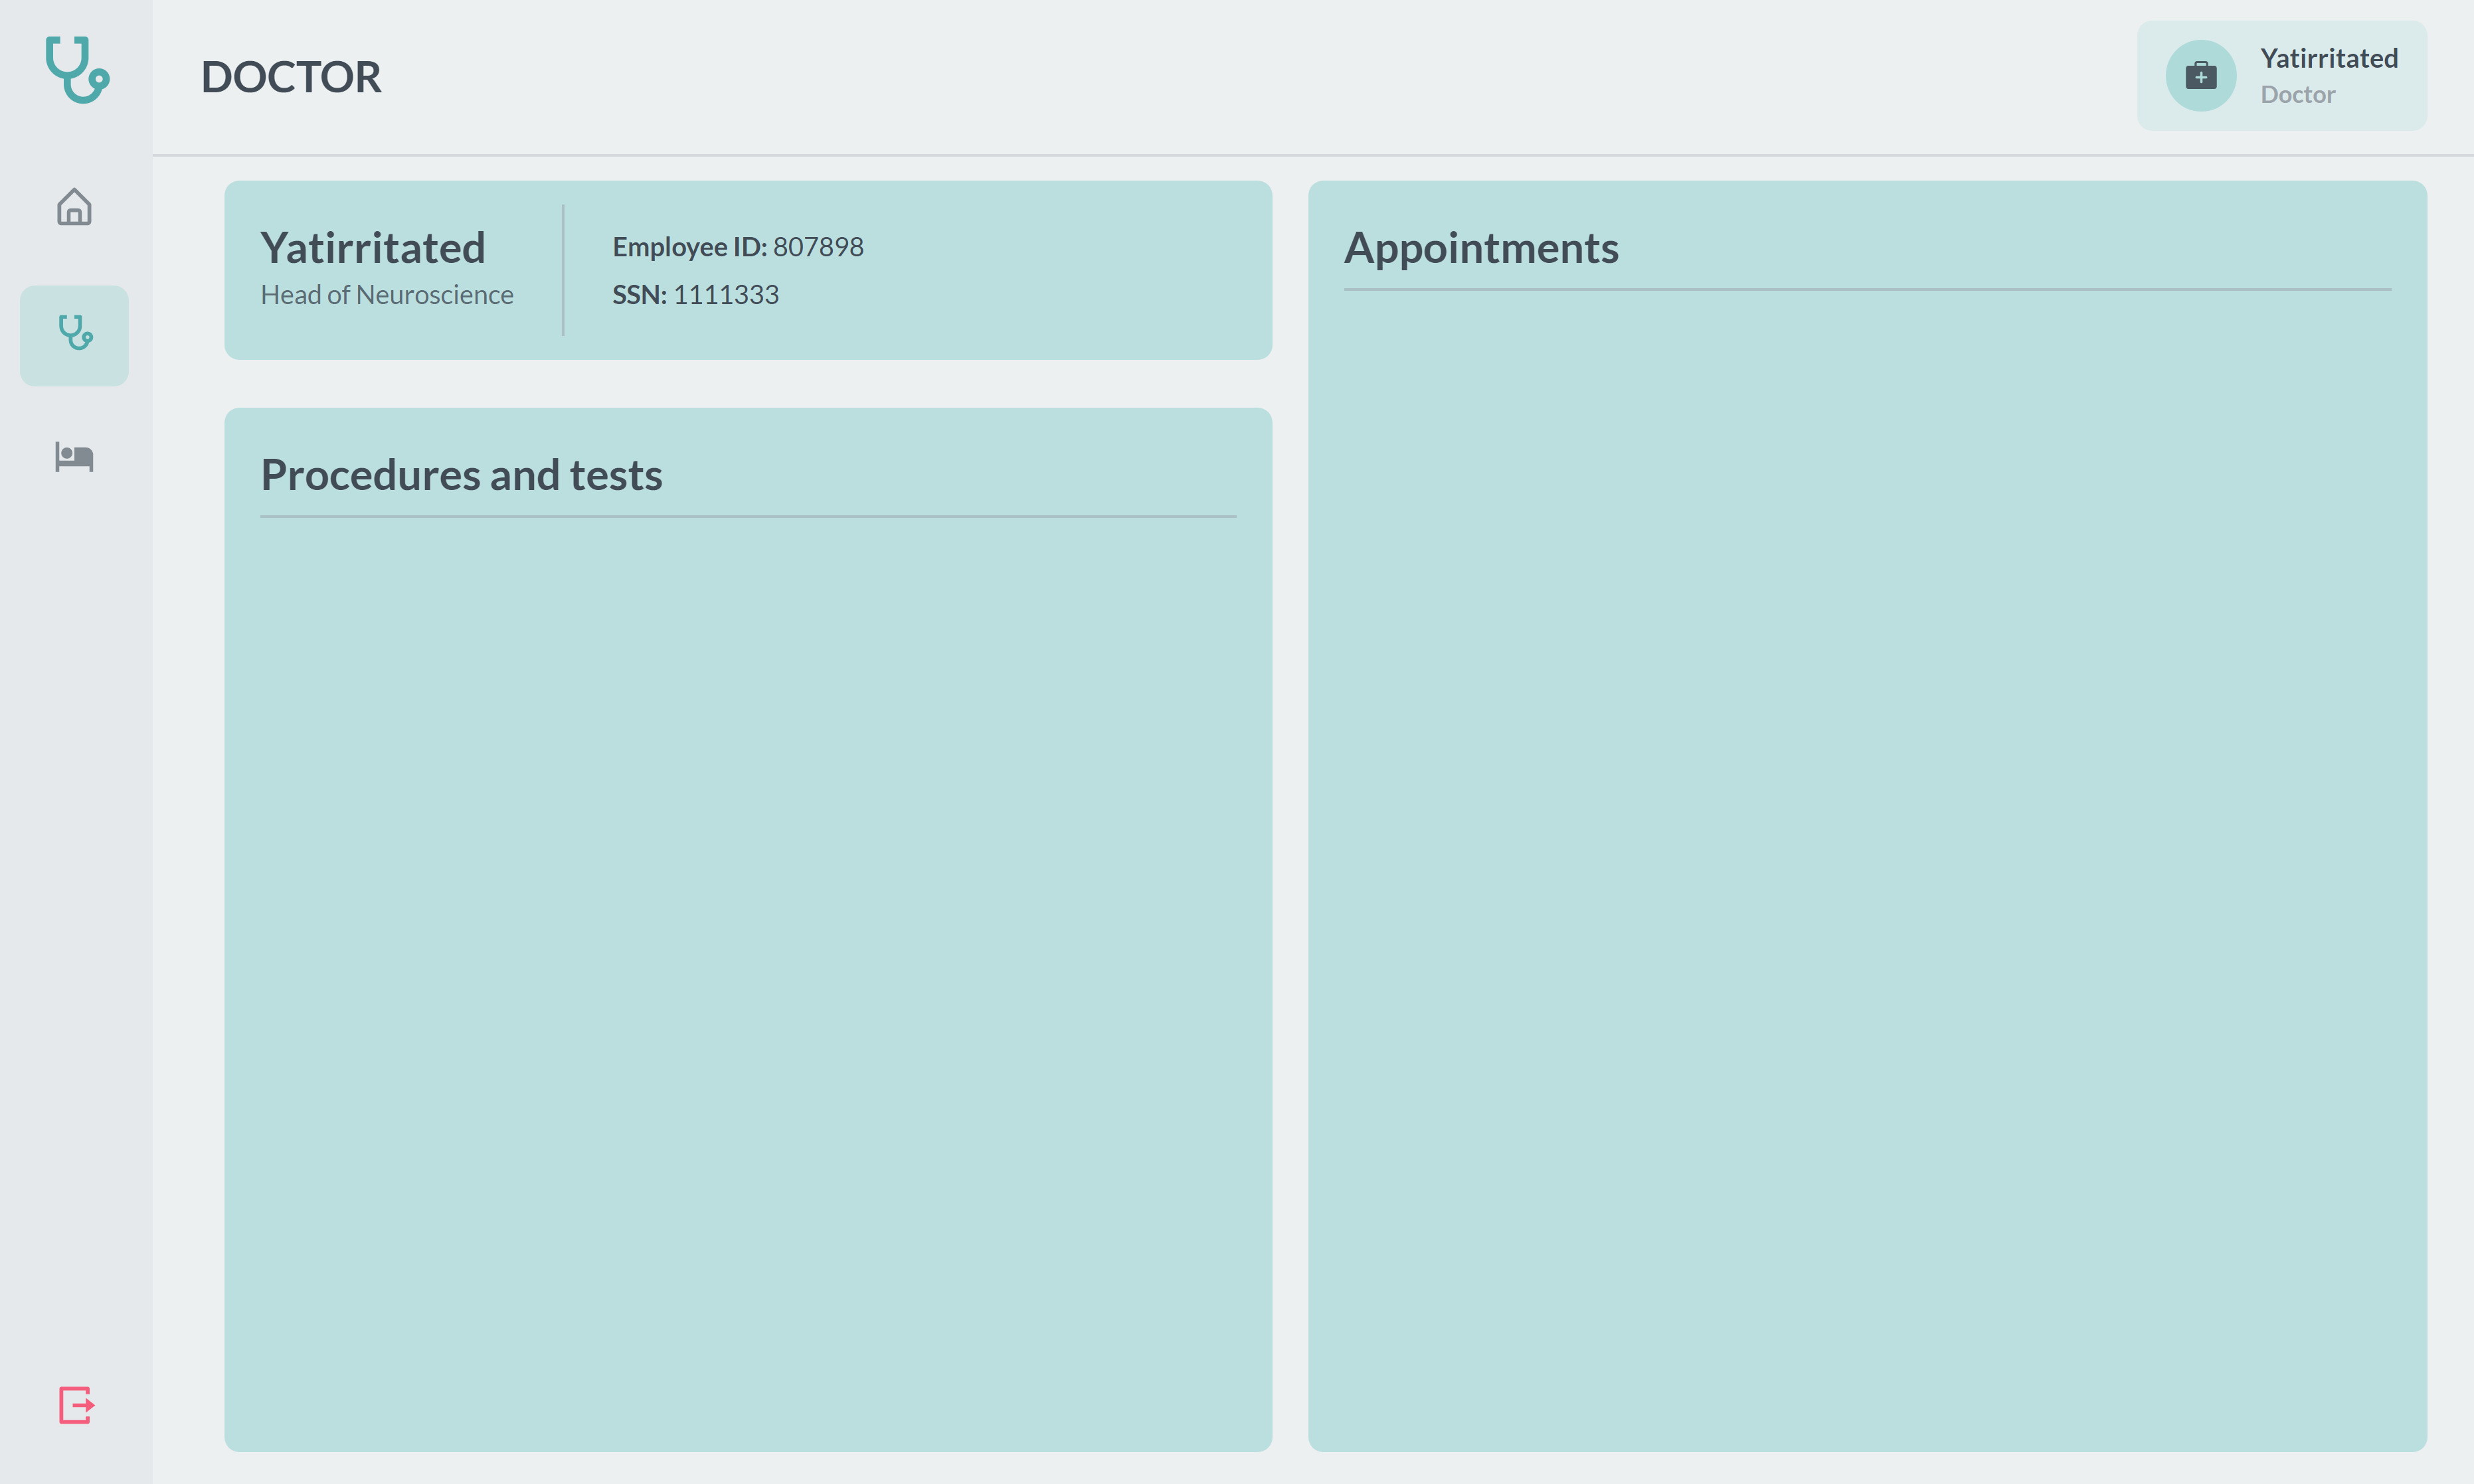
\includegraphics[width=1\textwidth]{new_doctor_board.png}
    \caption{New Doctor's Dashboard Page}
\end{figure}
\begin{figure}[htp]
    \centering
    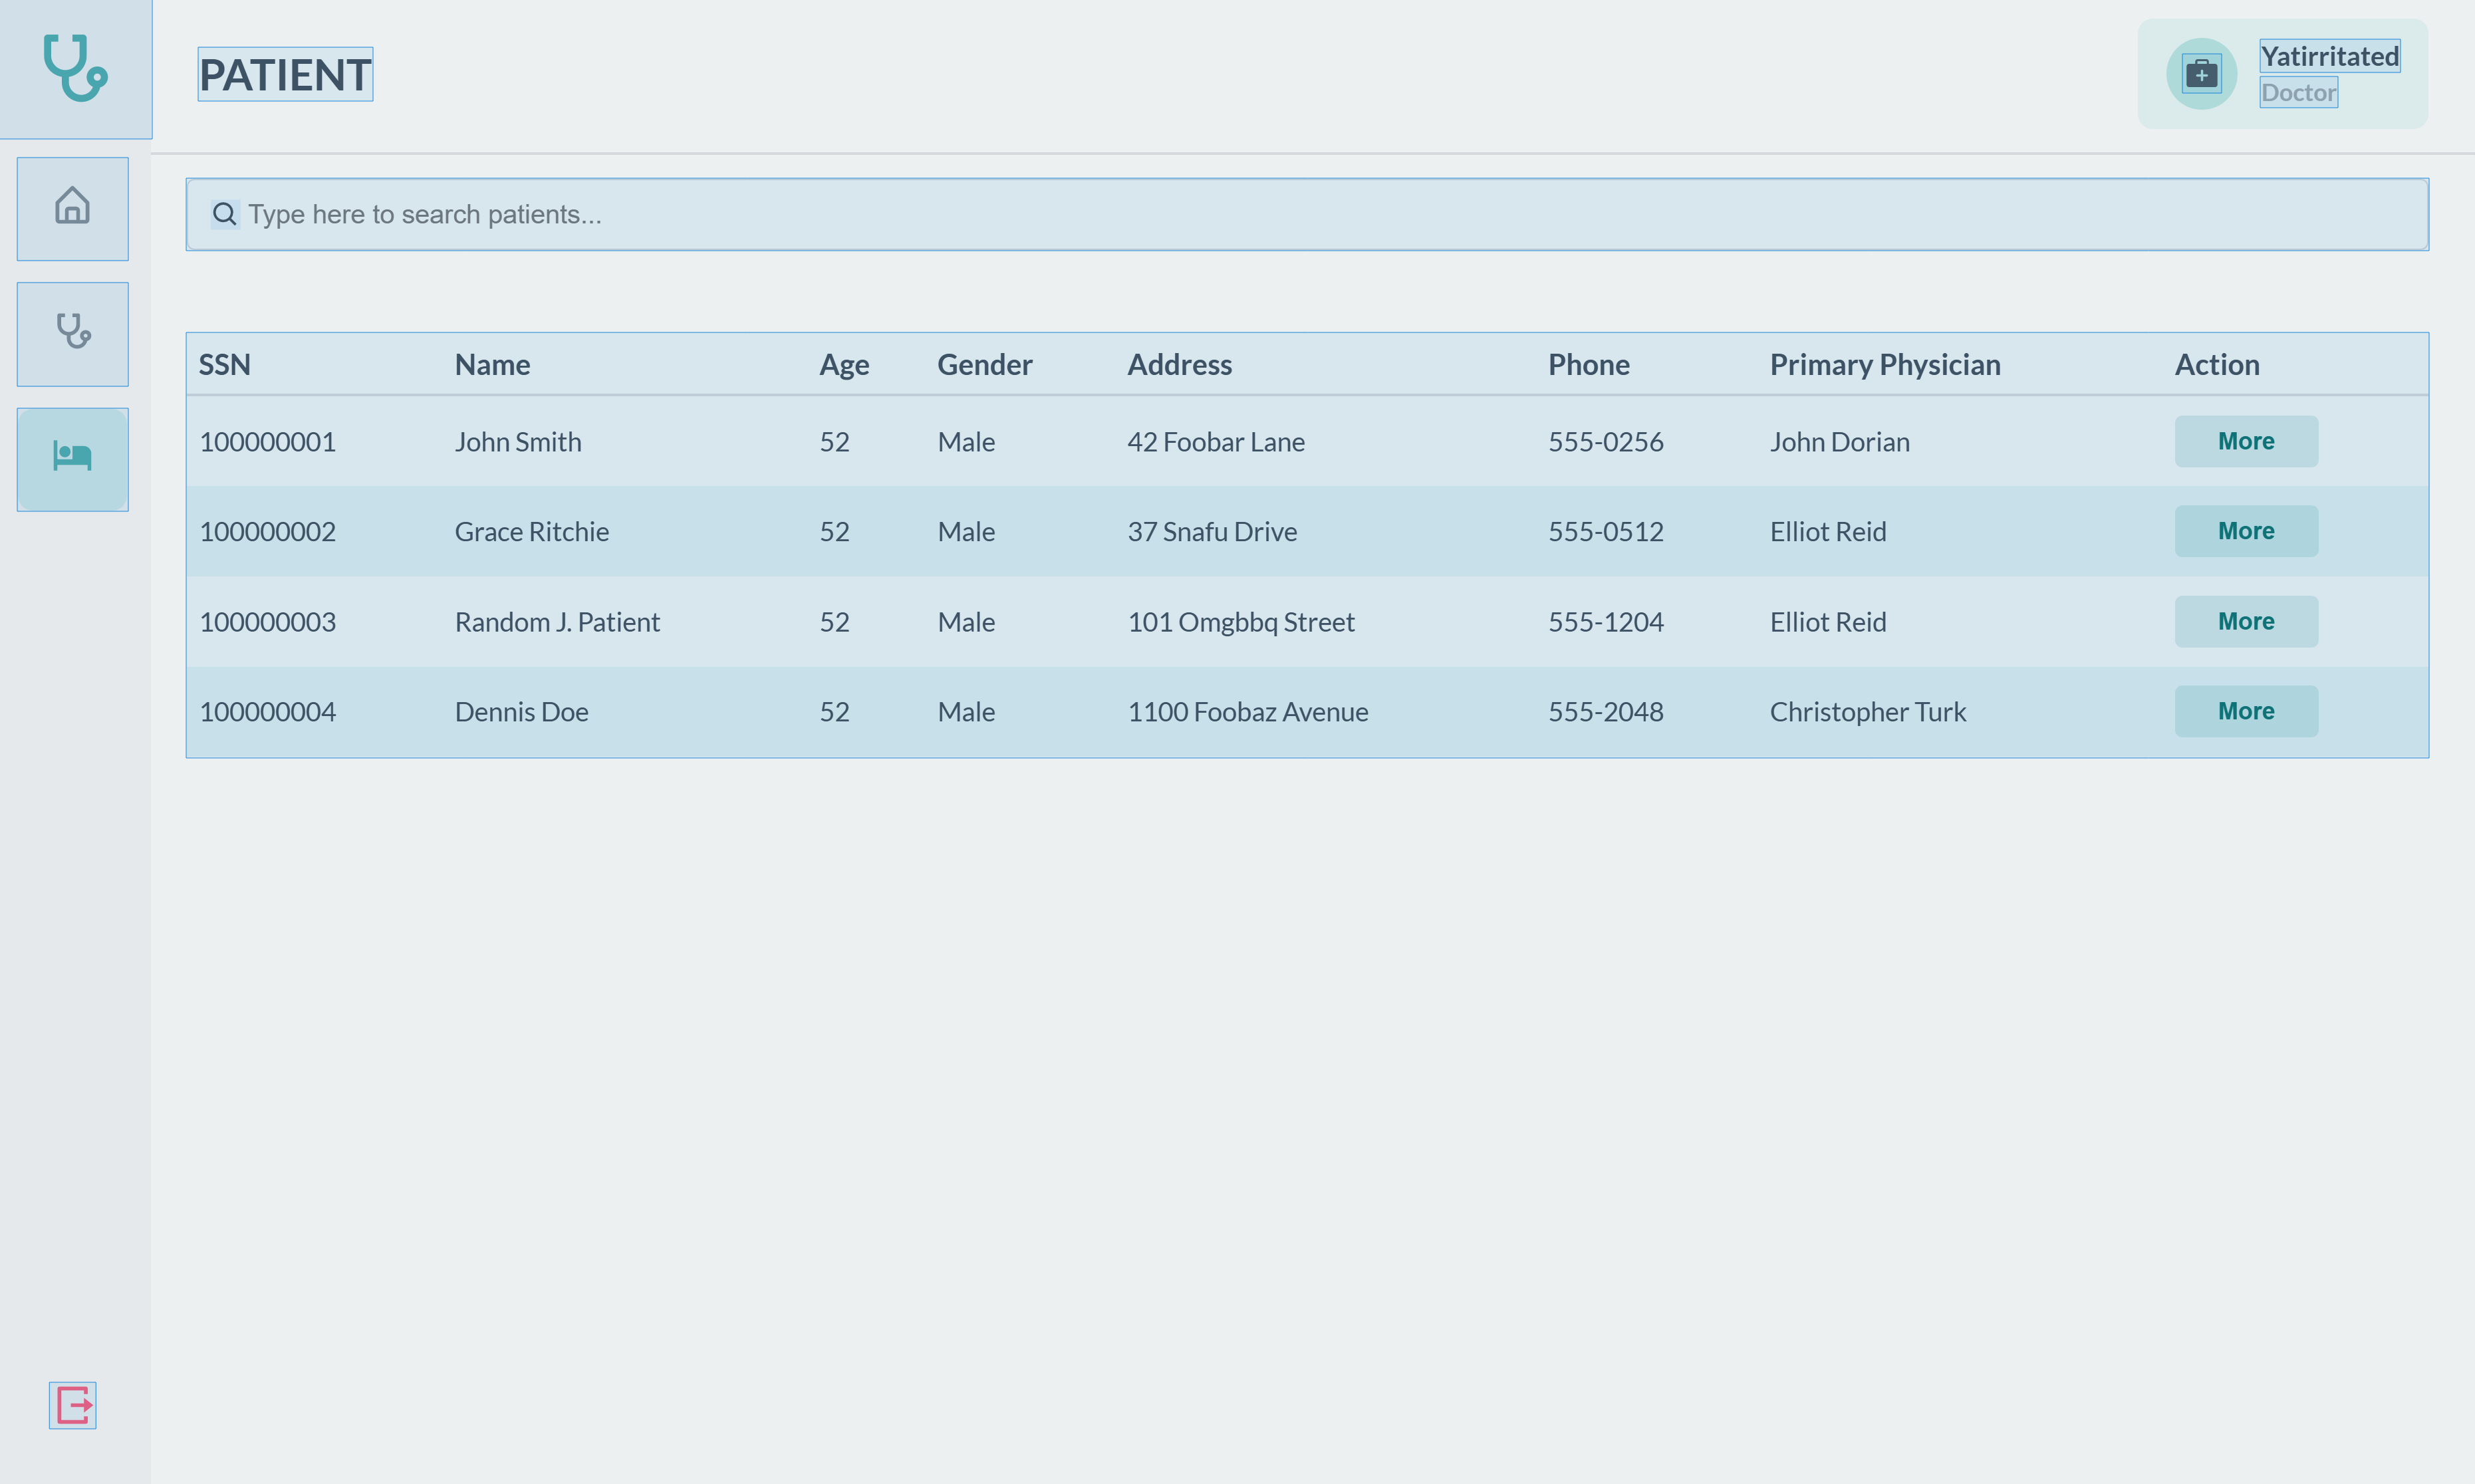
\includegraphics[width=1\textwidth]{patient_lookup.png}
    \caption{Patient Dashboard for Doctors Page}
\end{figure}
\begin{figure}[htp]
    \centering
    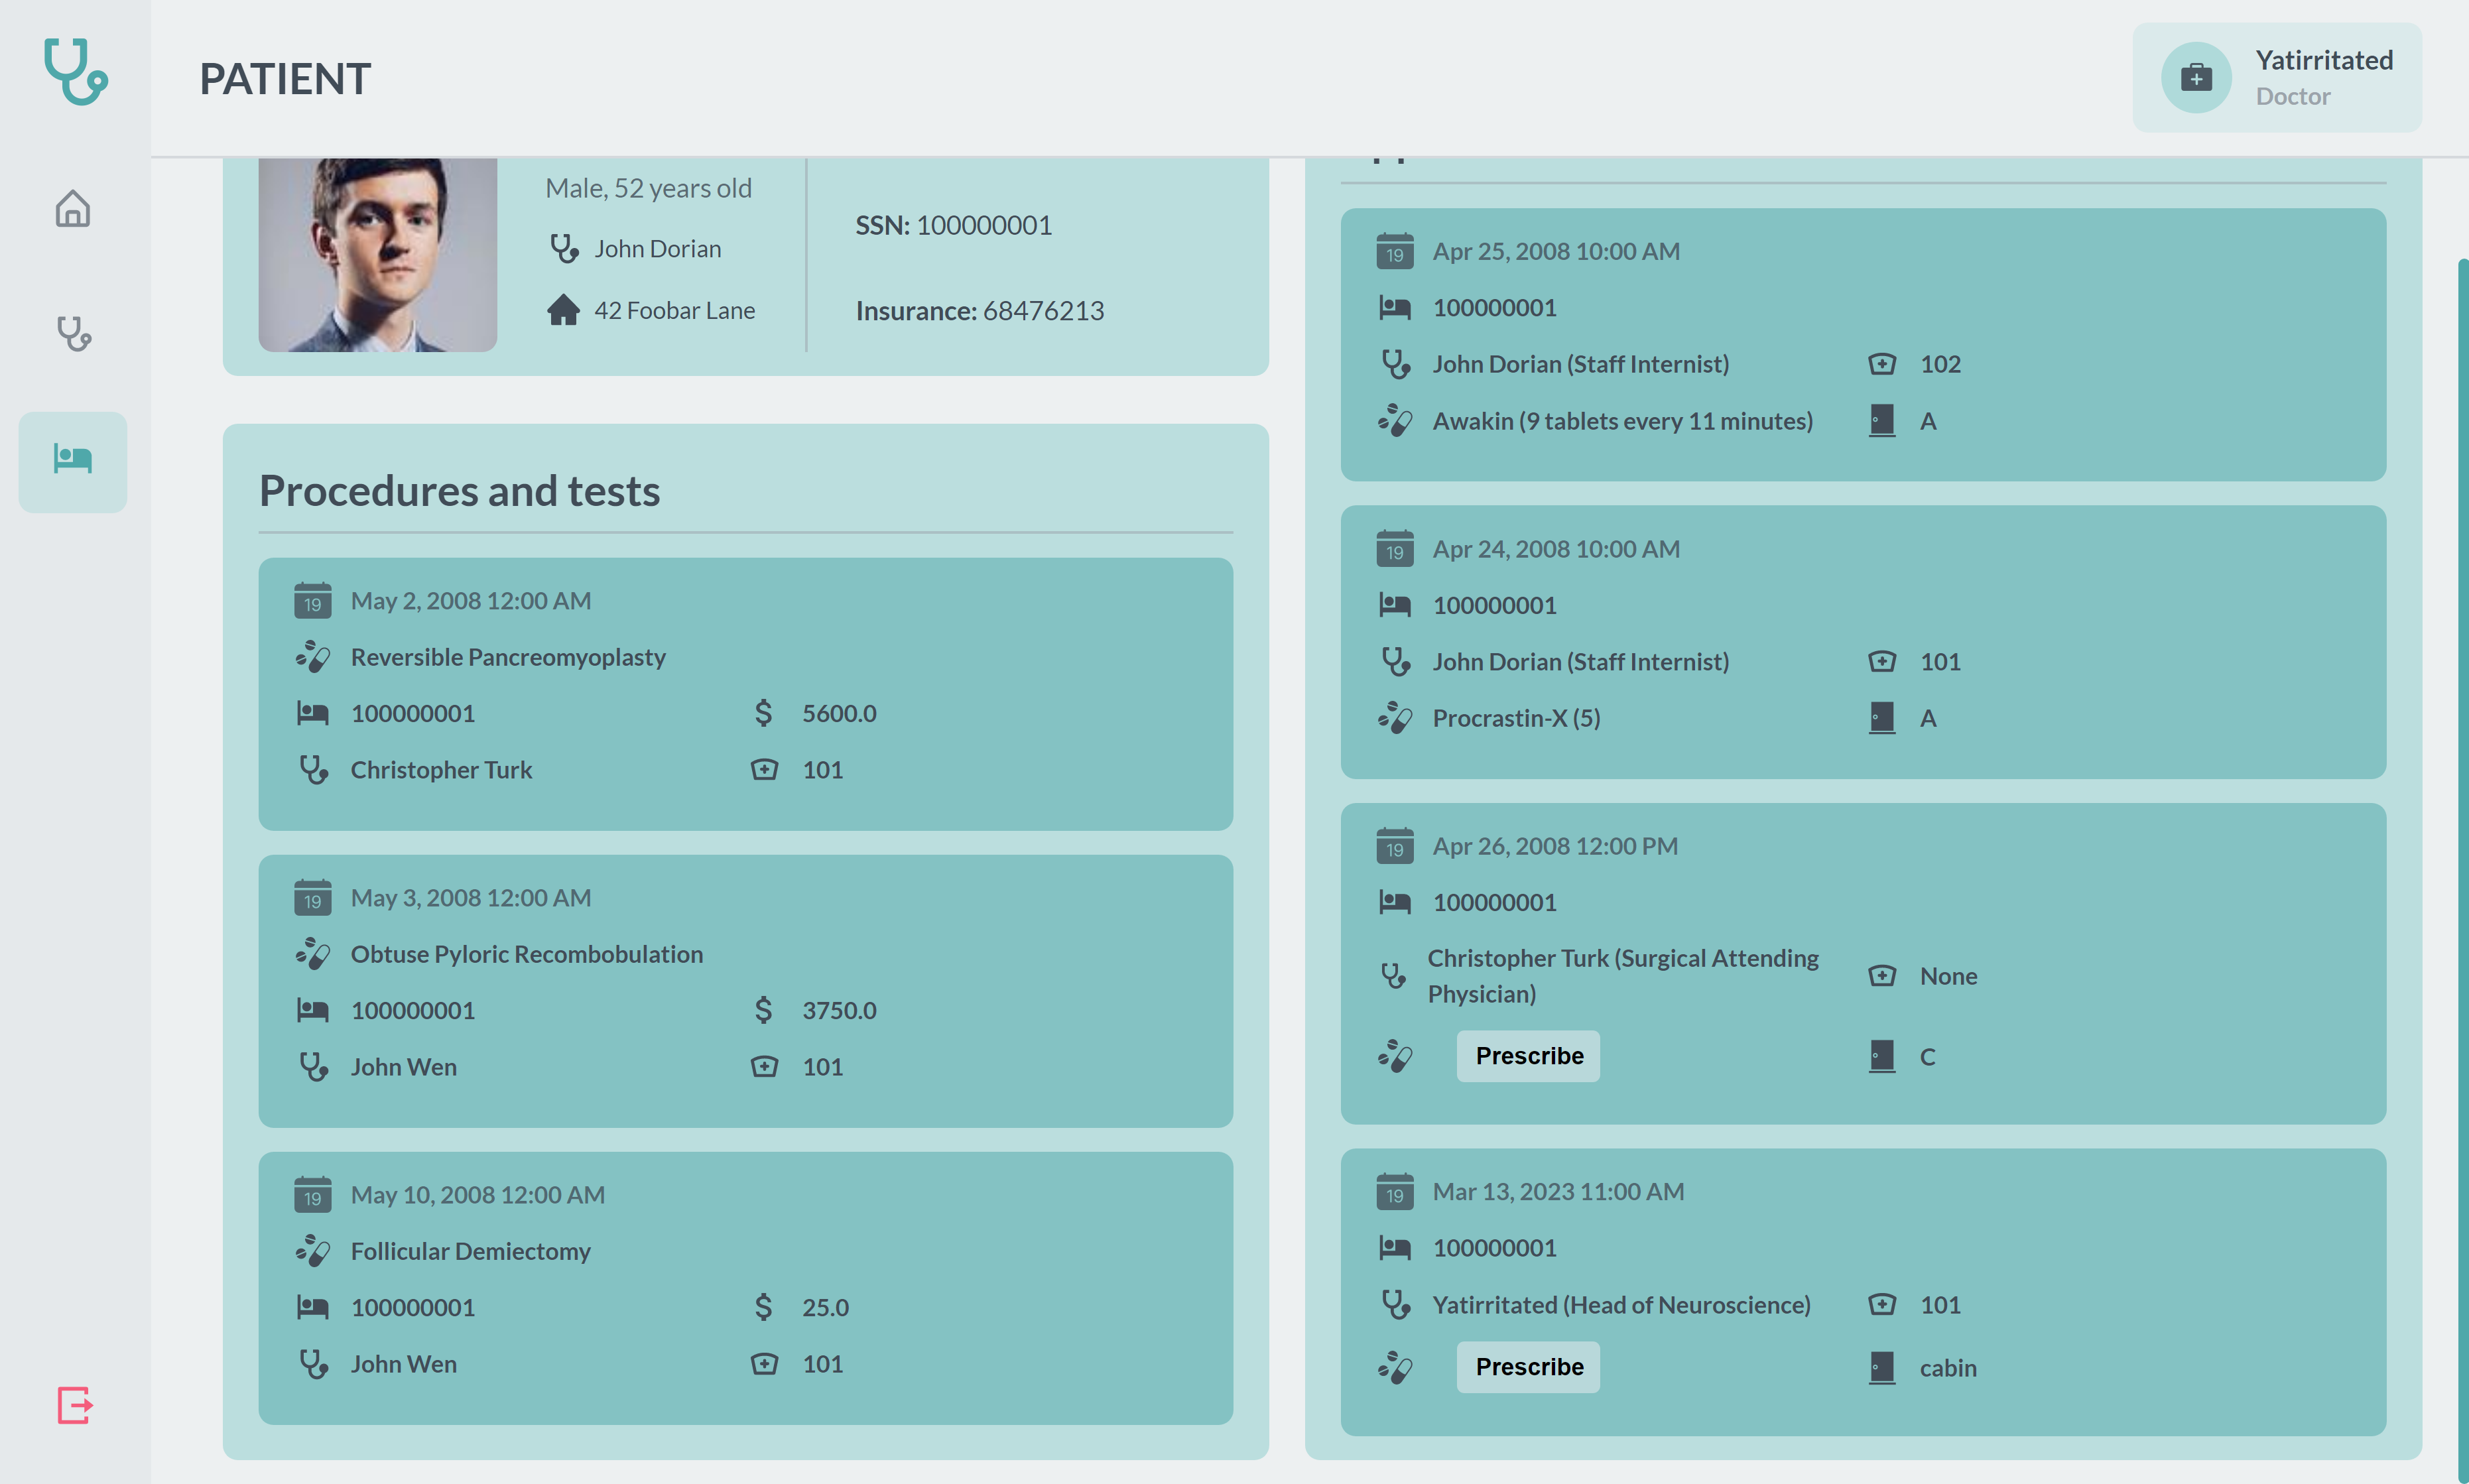
\includegraphics[width=1\textwidth]{pat_doc.png}
    \caption{Individual Patient as seen by Doctor}
\end{figure}
\begin{figure}[htp]
    \centering
    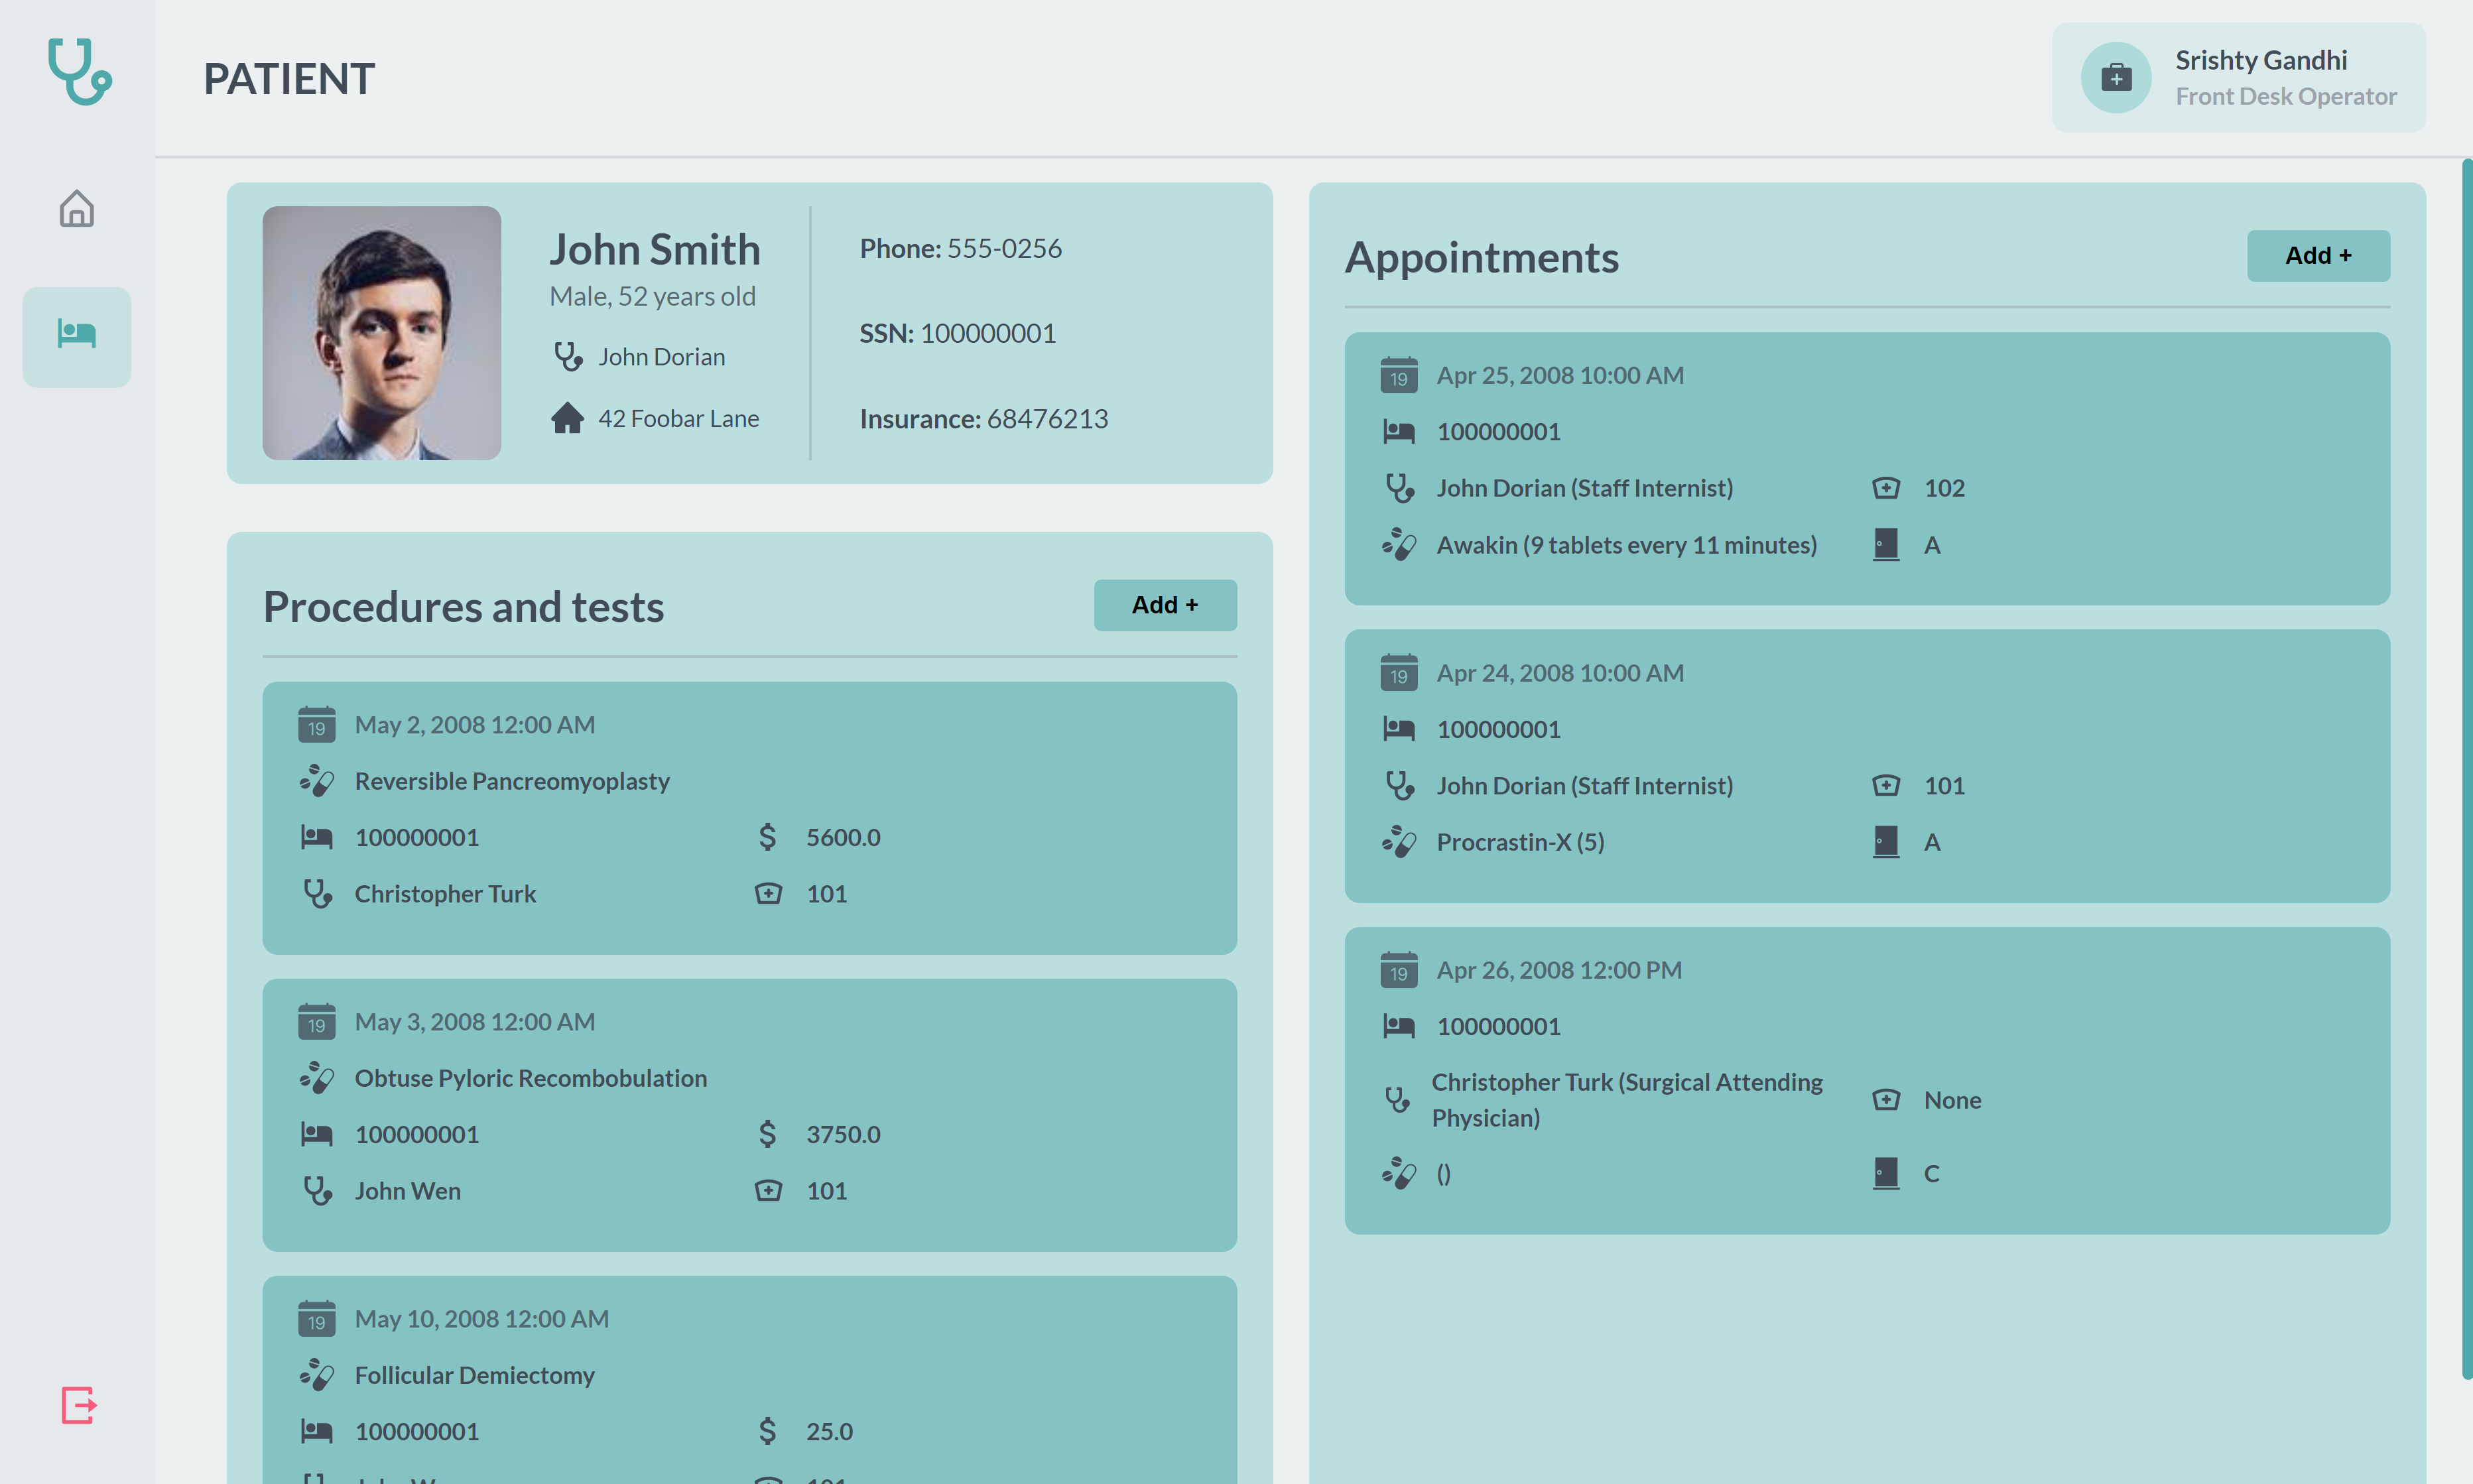
\includegraphics[width=1\textwidth]{patient_info.png}
    \caption{Individual Patient as seen by Front-Desk Operator}
\end{figure}
\begin{figure}[htp]
    \centering
    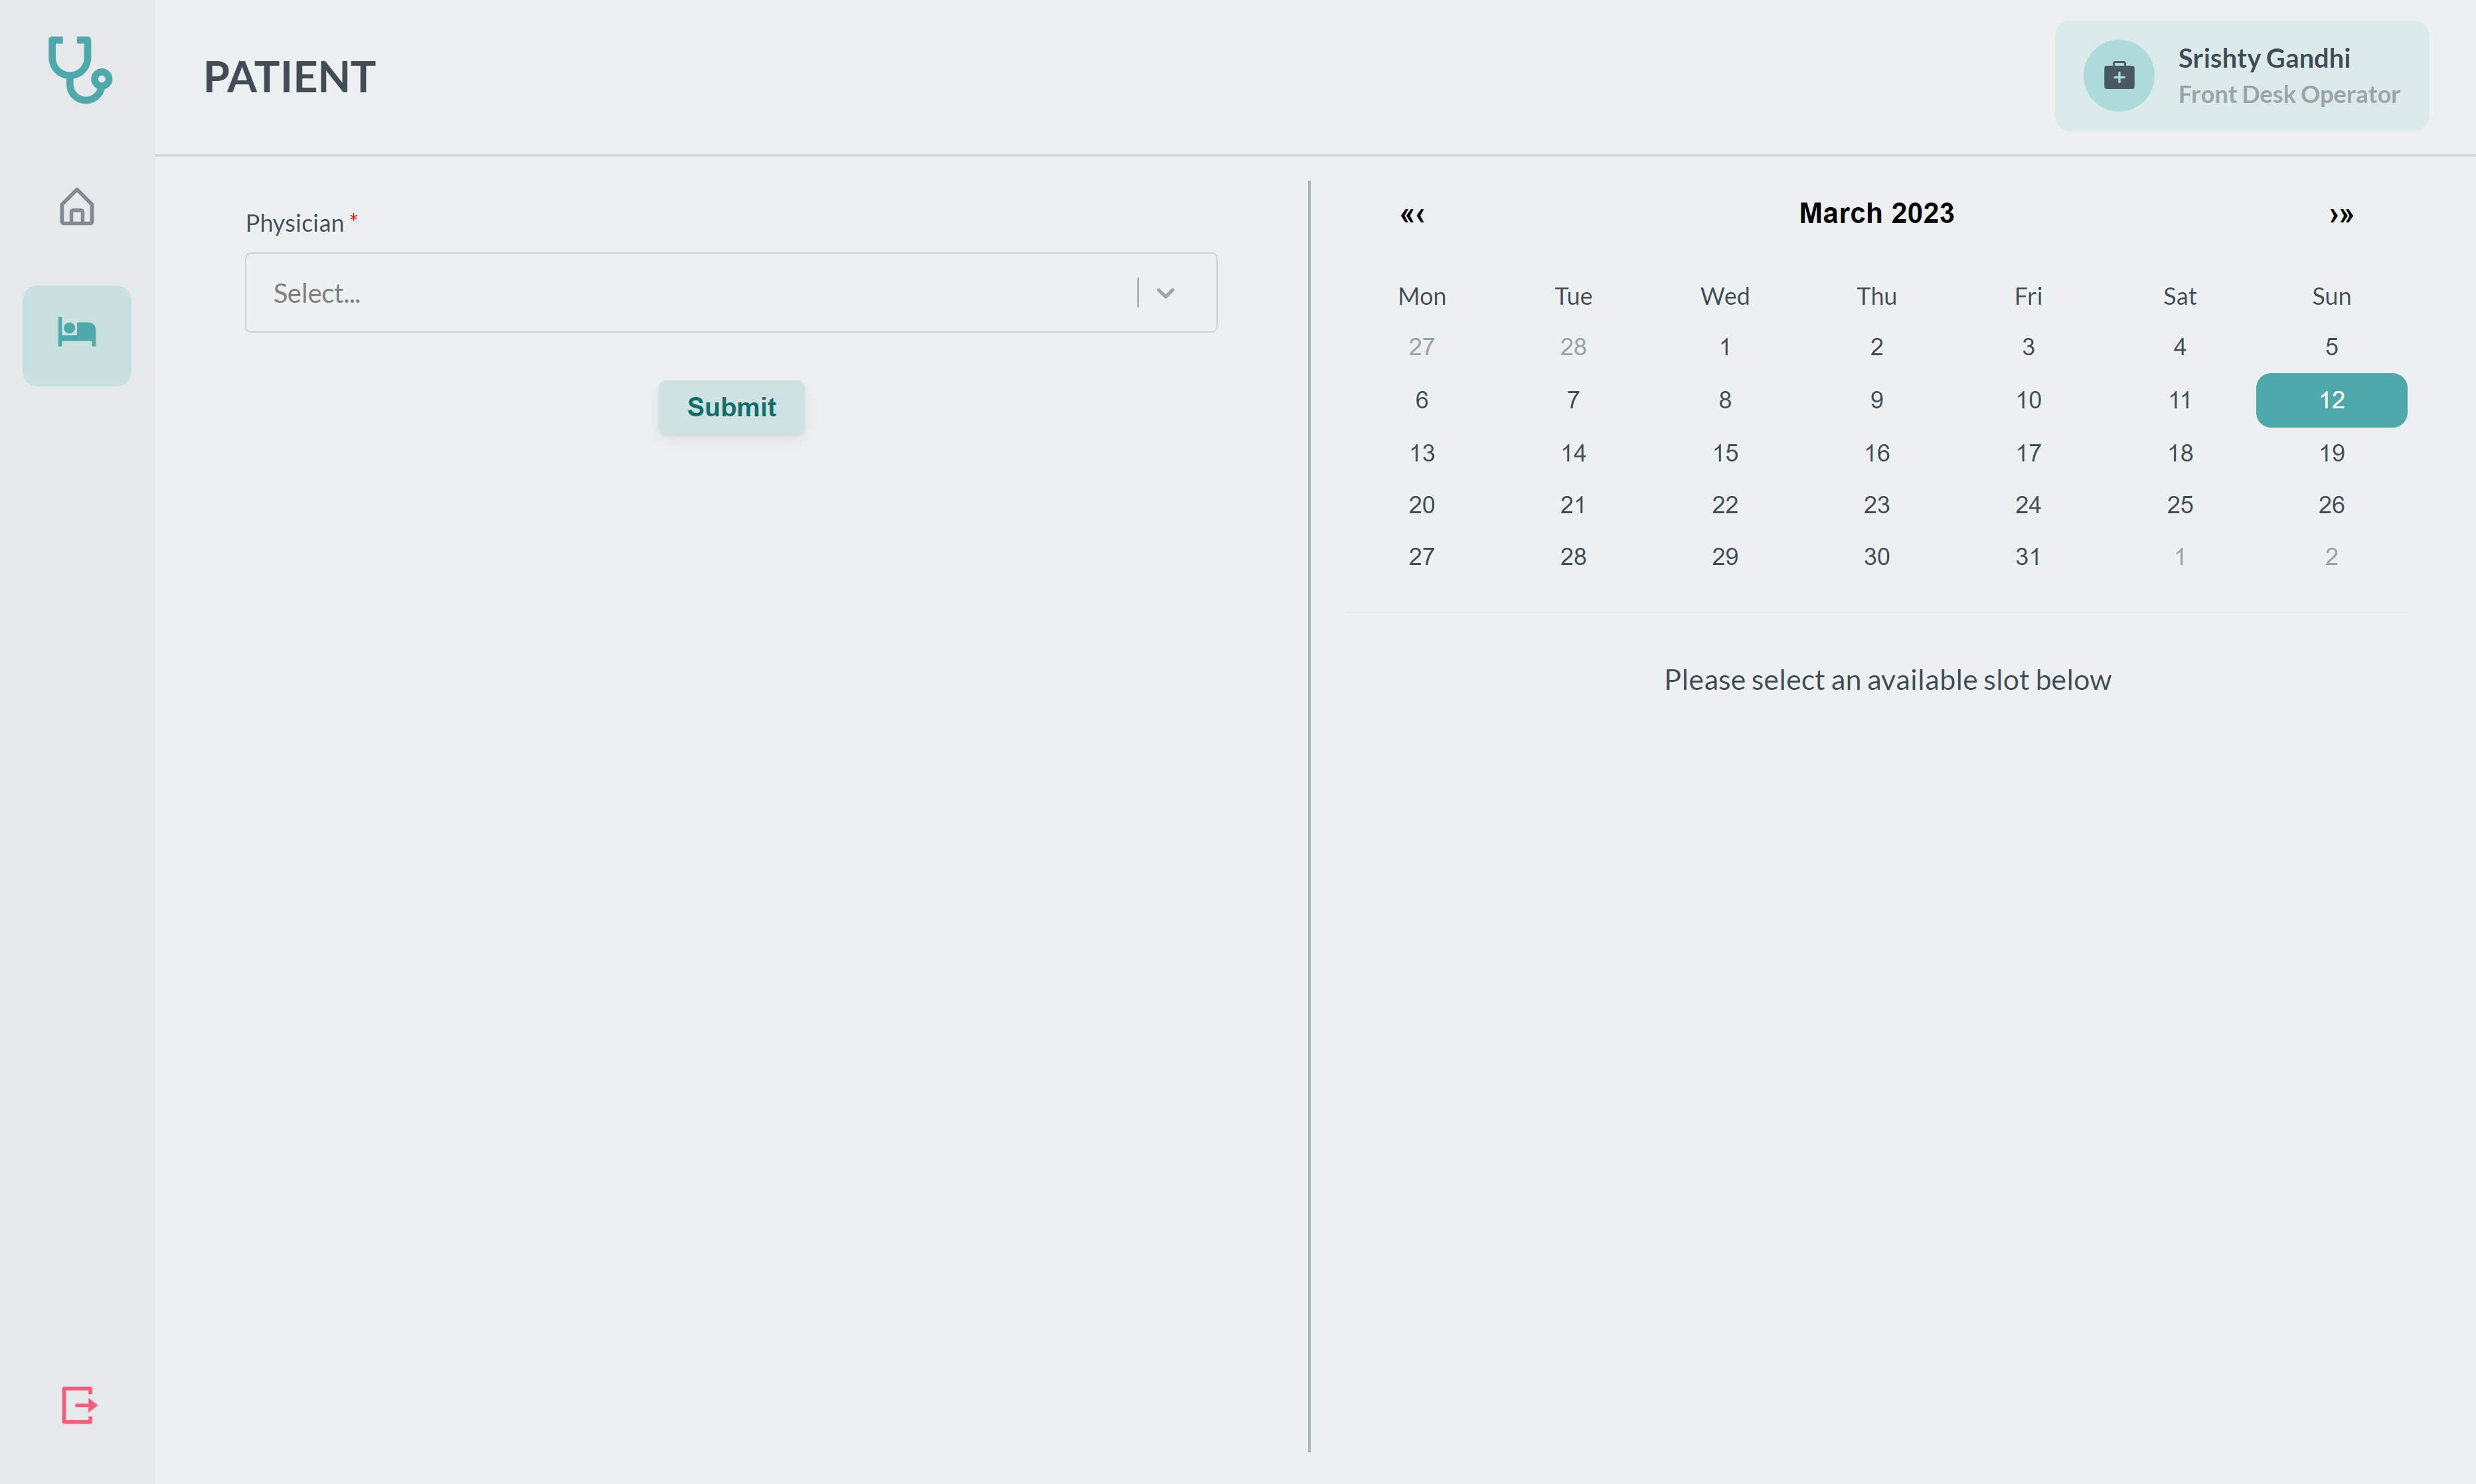
\includegraphics[width=1\textwidth]{appointment_sched.png}
    \caption{Appointment Scheduling by Front-Desk Operator}
\end{figure}
\begin{figure}[htp]
    \centering
    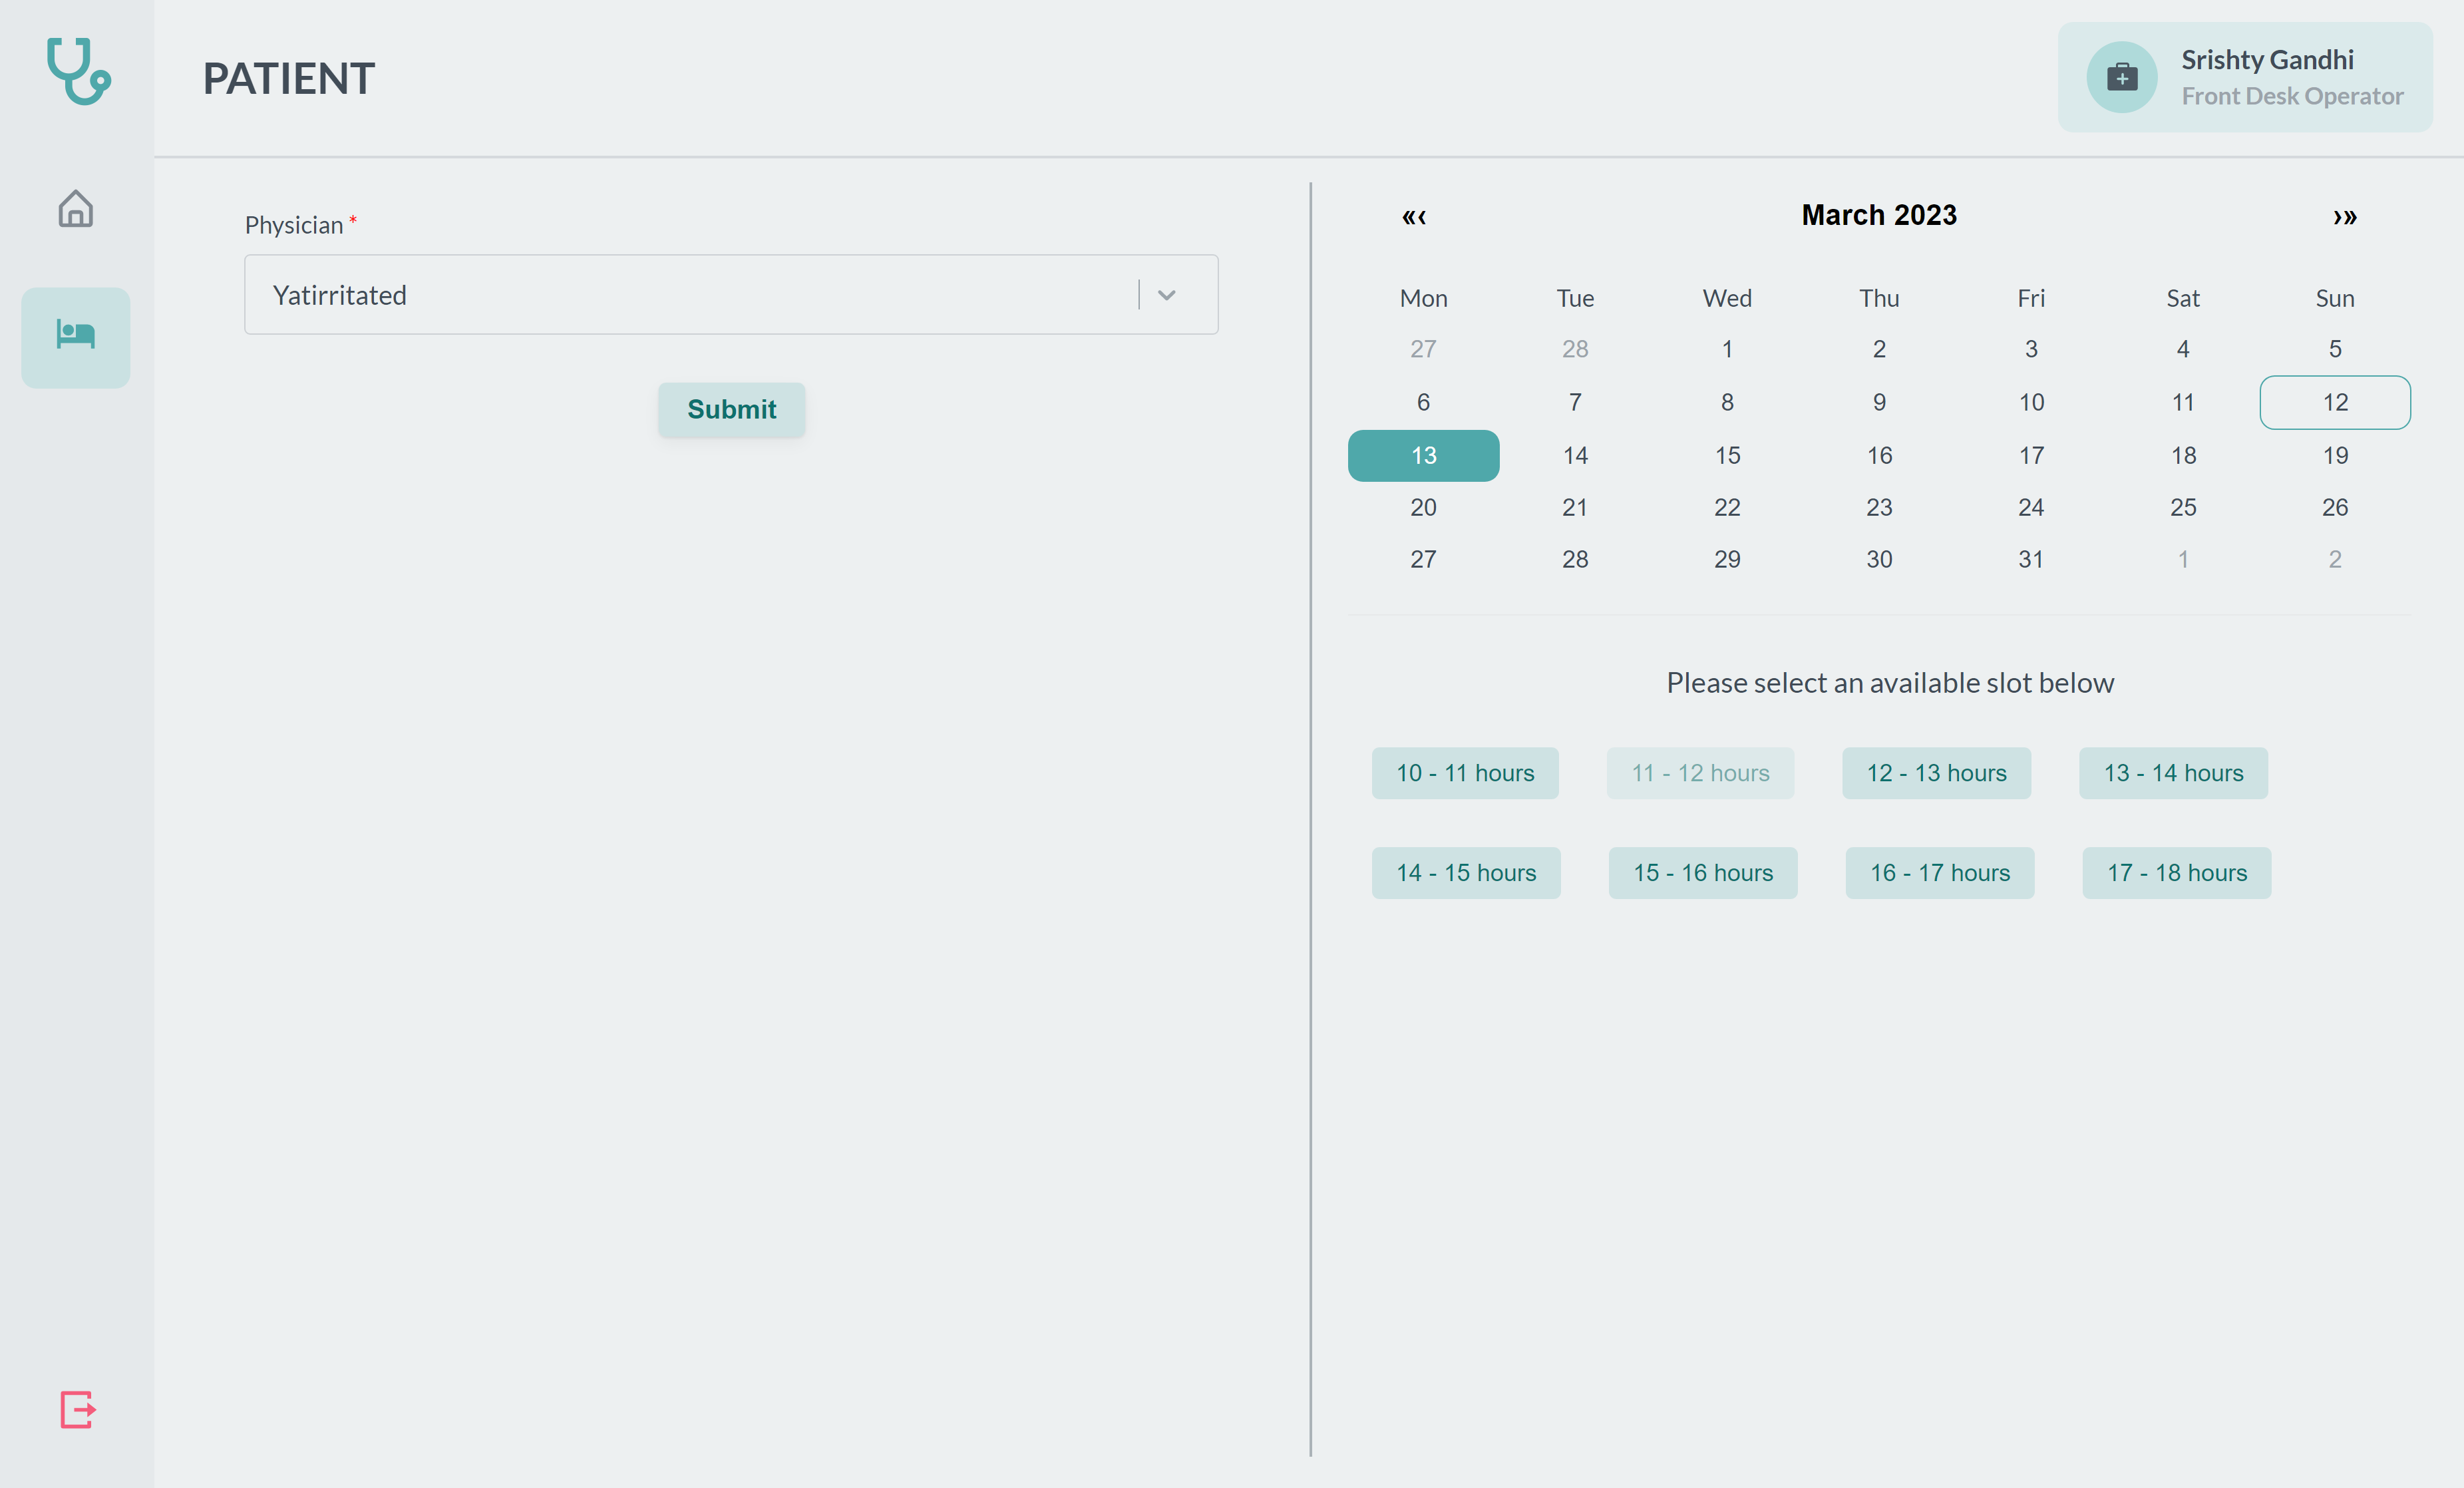
\includegraphics[width=1\textwidth]{appointment_for_a_doc.png}
    \caption{Appointment for a Doctor by Front-Desk Operator}
\end{figure}
\begin{figure}[htp]
    \centering
    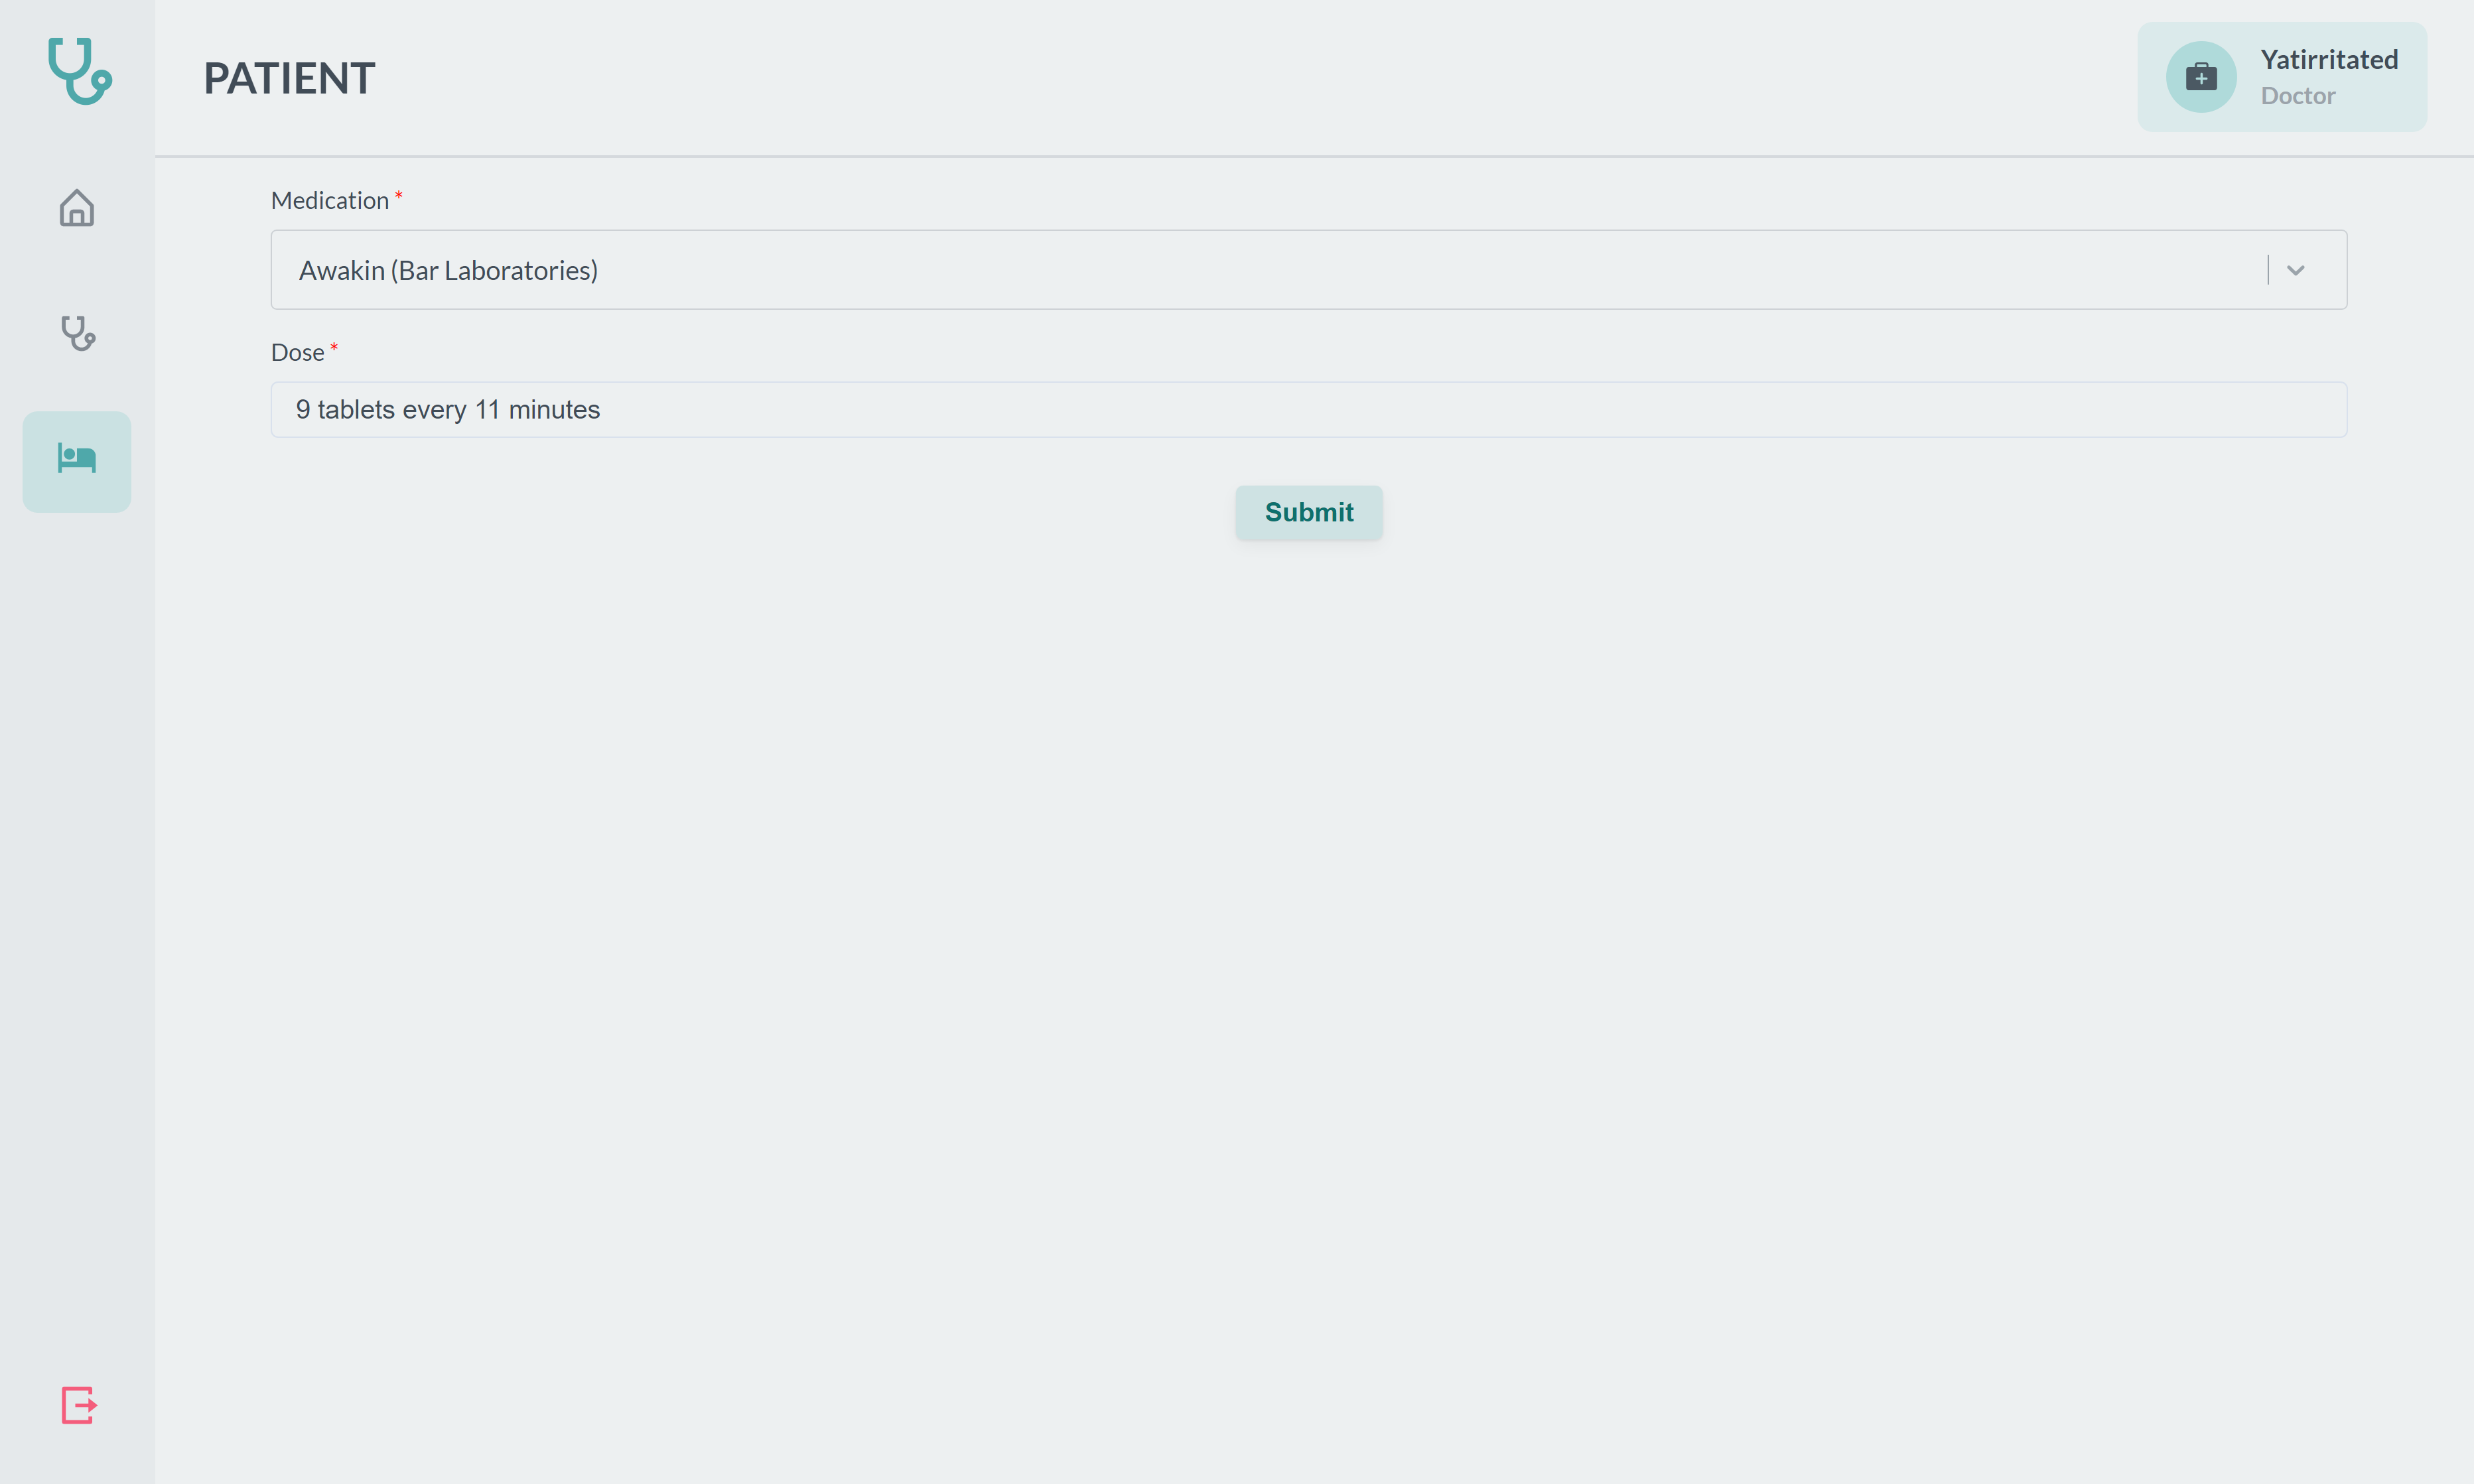
\includegraphics[width=1\textwidth]{prescribes.png}
    \caption{Prescribes view for a Doctor}
\end{figure}

\pagebreak
\item \textbf{Grid-Based Date Entry}
\\
In case of patient admission, appointment, and test scheduling, the 'Date' field is selected via a grid-UI. Hence no formatting, and logic errors can occur. 
\\
\\
Similarly for data consistency, if a 'Patient' or 'Date', which is not logically valid is selected, the system doesn't allow it. (For example, a patient, whose 'Stay' isn't ongoing, cannot have an appointment, or any appointment is unavailable or inconsistent (possibly a past time) then the system again doesn't allow it to happen.
\\
\item \textbf{Selection via Drop-Downs}
\\
The fields which are important as Foreign Keys are made available via a dropdown to select. Hence making it impossible to violate the existing conditions. (For example, the medications for an appointment).
\\
\item \textbf{In Case of Issues (Like Unavailable Room)}
\\
In case of issues that come apparent later during the process, an error is shown as an alert denoting the issue. (for example, a patient, when added, by logic is given a room automatically, in case none is available, we can acknowledge the same).
\end{enumerate}


\newpage
  





% \section{Literature review}\label{sec:lit-rev}

% \lipsum[3-4]\cite{einstein}

% \section{Methodology}\label{sec:meth}

% \lipsum[5-6]\cite{latexcompanion}

% \section{Results}\label{sec:res}

% \lipsum[7-8]\cite{knuthwebsite}

% %===========================================================
% %===========================================================

% \bibliographystyle{ieeetr}
% \bibliography{refs}


\end{document} 
